\documentclass[12pt,a4paper]{article}

\usepackage{fontspec}
\usepackage{polyglossia}
\usepackage{geometry}
\usepackage{setspace}
\usepackage{indentfirst}
\usepackage{hyperref}
\usepackage{enumitem}
\usepackage{amsmath}
\usepackage{amssymb}
\usepackage{array}
\usepackage{float}
\usepackage{multirow}
\usepackage{caption}
\usepackage{subcaption}
\usepackage{graphicx}
\usepackage{tikz}
\usetikzlibrary{arrows.meta,positioning}

\setmainlanguage{russian}
\setotherlanguage{english}
\setmainfont{Times New Roman}
\newfontfamily\cyrillicfont{Times New Roman}
\newfontfamily\cyrillicfontsf{Times New Roman}
\newfontfamily\cyrillicfonttt{Courier New}
\renewcommand{\contentsname}{Оглавление}
\renewcommand{\refname}{Литература}

\DeclareCaptionLabelSeparator{dash}{ — }
\captionsetup[figure]{name=Рисунок,labelsep=dash,justification=centering}
\captionsetup[table]{name=Таблица,labelsep=dash,justification=raggedright,singlelinecheck=false}

\makeatletter
\renewcommand*\l@section{\@dottedtocline{1}{0em}{2.4em}}
\renewcommand*\l@subsection{\@dottedtocline{2}{1.5em}{3.6em}}
\renewcommand*\l@subsubsection{\@dottedtocline{3}{4.8em}{4.4em}}
\makeatother

\geometry{
    left=30mm,
    right=15mm,
    top=20mm,
    bottom=20mm
}

\onehalfspacing
\hypersetup{
    colorlinks=true,
    linkcolor=black,
    urlcolor=black,
    citecolor=black,
    pdfauthor={Э. Э. Кадыров},
    pdftitle={Прогноз космологического красного смещения по фотометрическим признакам}
}

\newcommand{\worktitle}{Прогноз космологического красного смещения по фотометрическим признакам}
\newcommand{\studentname}{Кадыров Эркин Энверович}
\newcommand{\faculty}{Факультет вычислительной математики и кибернетики}
\newcommand{\department}{Кафедра информационных интеллектуальных технологий}
\newcommand{\worktype}{КУРСОВАЯ РАБОТА}
\newcommand{\supervisorslabel}{Научные руководители}
\newcommand{\supervisor}{к.\,ф.-м.\,н. Мещеряков А.\,В.\\Герасимов С.\,В.}
\newcommand{\workyear}{2026}

\begin{document}

\begin{titlepage}
    \thispagestyle{empty}

    \begin{center}
        \vspace*{1cm}

        \includegraphics[width=0.32\textwidth]{msu.jpg}

        \vspace{1cm}

        {\large Московский государственный университет имени М.\,В. Ломоносова\par}
        \vspace{0.3cm}
        {\large \faculty\par}
        \vspace{0.3cm}
        {\large \department\par}

        \vspace*{32mm}

        {\large \studentname\par}

        \vspace{20mm}

        {\Large \worktitle\par}

        \vspace{25mm}

        {\large \worktype\par}

        \vfill
    \end{center}

    \begin{flushright}
        \begin{minipage}{0.45\textwidth}
            \raggedright
            \supervisorslabel:\\[0.3cm]
            \supervisor
        \end{minipage}
    \end{flushright}

    \vfill

    \begin{center}
        Москва, \workyear
    \end{center}
\end{titlepage}

\section*{Аннотация}
\addcontentsline{toc}{section}{Аннотация}

В работе рассматривается задача прогнозирования фотометрического красного смещения астрономических объектов, в том числе рентгеновских источников, по широкополосным фотометрическим признакам. Актуальность задачи связана с ростом объема обзоров неба и необходимостью оценивать красные смещения для больших каталогов без спектроскопии. В тексте рассмотрены причины сложности задачи, наборы данных Teddy, Happy и SRGz, методы классического и глубокого обучения, а также экспериментальный стенд. Эксперименты показывают падение качества классических моделей при сдвиге распределения, фотометрическом шуме и смещении к среднему.

\textbf{Ключевые слова:} ФОТОМЕТРИЧЕСКОЕ КРАСНОЕ СМЕЩЕНИЕ, МАШИННОЕ ОБУЧЕНИЕ, ГЛУБОКОЕ ОБУЧЕНИЕ, РЕНТГЕНОВСКИЕ ИСТОЧНИКИ, TEDDY, HAPPY, SRGZ, CONVNEXT, CAPSNET.

\newpage
\tableofcontents
\newpage

\section*{Введение}
\addcontentsline{toc}{section}{Введение}

Космологическое красное смещение представляет собой наблюдаемое увеличение длины волны излучения удаленных астрономических объектов, обусловленное расширением Вселенной. Эта величина играет ключевую роль в современной наблюдательной космологии, поскольку позволяет оценивать расстояния до объектов, восстанавливать трехмерную структуру Вселенной и анализировать ее эволюцию на разных эпохах. Для объектов с большим красным смещением наблюдатель фактически получает информацию о более ранних стадиях развития Вселенной, поэтому точность его оценки напрямую влияет на качество астрофизических выводов.

Объем астрономических данных растет за счет крупных обзоров неба, таких как SDSS, DESI и LSST. Это делает задачу массовой оценки красных смещений особенно важной. Спектроскопия дает более точный результат, но требует больших затрат на каждый объект. Фотометрия позволяет работать с большими каталогами, но приводит к более сложной задаче регрессии.

Актуальность фотометрического определения красного смещения подтверждается современными обзорами литературы. В частности, в работе J. A. Newman и D. Gruen отмечается, что фотометрические красные смещения являются одним из базовых элементов научной программы обзоров следующего поколения~\cite{newman2022}. Они необходимы для изучения крупномасштабной структуры Вселенной, оценки светимости и массы объектов, а также для решения задач, связанных с темной энергией и космологическими параметрами.

Отдельный интерес представляет прогноз фотометрического красного смещения для рентгеновских источников: активных ядер галактик, квазаров, черных дыр и скоплений галактик. Для российской астрономии задача связана с обзором СРГ/eROSITA. В работе А. Мещерякова и соавторов представлен каталог оптических компаньонов точечных рентгеновских источников и методы его анализа~\cite{meshcheryakov2022}.

Таким образом, работа находится на пересечении астрофизики, анализа данных и машинного обучения.

\newpage
\section{Постановка задачи}

В работе решается задача исследования и разработки алгоритмов машинного и глубокого обучения для предсказания фотометрического красного смещения рентгеновских источников.

Входными данными являются фотометрические признаки объектов из астрономических обзоров. Для части нейросетевых экспериментов дополнительно рассматриваются изображения объектов в нескольких фильтрах, поскольку они содержат морфологическую и пространственную информацию. Целевая переменная — красное смещение, полученное по спектроскопическим наблюдениям.

\newpage
\section{Обзор литературы и существующих решений}
\label{sec:review}

Обзор нужен, чтобы выбрать методы и сценарии эксперимента, отвечающие на основной вопрос работы: какие подходы устойчивее в задаче фотометрического красного смещения при сдвиге распределения, шуме наблюдений и смещении к среднему. Структура обзора: особенности задачи, наборы данных, классические табличные алгоритмы, архитектуры глубокого обучения на изображениях, метрики качества и итоговые выводы.

Критерии сравнения методов выбраны под особенности photoz, описанные ниже:
\begin{itemize}
    \item \emph{тип входных данных} — табличные фотометрические признаки или многоканальные изображения. Изображения дополнительно несут морфологию и распределение яркости, поэтому потенциальная точность у моделей с разным типом входа разная.

    \item \emph{поведение при сдвиге распределения}. Спектроскопическая обучающая выборка отличается от полной фотометрической, поэтому важно не качество интерполяции, а поведение при экстраполяции в редко представленные области признакового пространства. Проверяется тестом Teddy~\cite{beck2017}.

    \item \emph{устойчивость к фотометрическому шуму}. Уровень шума растет к слабым источникам, и модель, обученная на ярких объектах, применяется к более шумным. Проверяется тестом Happy~\cite{beck2017}, в котором подвыборки различаются уровнем добавленного шума.

    \item \emph{вычислительная стоимость обучения и применения}. Каталоги LSST, Euclid и СРГ содержат десятки миллионов и миллиарды объектов, поэтому метод, требующий значимых ресурсов на объект, не масштабируется.

    \item \emph{метрики $\sigma_{NMAD}$, $f_{\mathrm{outlier}}$ и $\mathrm{bias}$}. Средняя квадратичная ошибка усредняет типичные и катастрофические промахи и не показывает смещения. Принятая в астрономии тройка контролирует масштаб ошибки, долю выбросов и систематическое смещение независимо.
\end{itemize}

\subsection{Особенности задачи фотометрического красного смещения}
\label{sec:photoz-challenges}

Принципиальная сложность задачи photoz связана с тем, что обучающая и применяемая выборки имеют разную природу. Спектроскопические наблюдения проводятся избирательно: для них выбираются объекты с заранее известной приблизительной светимостью и достаточной фотометрической яркостью, попадающие в программу конкретного обзора. Поэтому спектроскопическая подвыборка систематически отличается от полной фотометрической как по яркости, так и по красному смещению~\cite{newman2022}. На практике это означает, что модель, обученная на «доступных» источниках, должна затем применяться к «недоступным» — более слабым, более далеким и хуже представленным в обучении объектам. Эта разница не является случайным шумом: она структурно встроена в способ получения спектроскопических меток.

Хорошей иллюстрацией ситуации служит каталог SRGz~\cite{meshcheryakov2022}, на основе которого формируется одна из задач данной работы. На рисунке~\ref{fig:srgz-distribution} приведено распределение спектроскопических красных смещений рентгеновских источников из этого каталога с разделением по типу объекта. Распределение $z_\mathrm{spec}$ сильно неравномерно: основной пик приходится на квазары с $z \approx 1$, галактики локализованы в области $z \lesssim 0{,}5$, а на больших красных смещениях, начиная с $z \gtrsim 3$, объектов на несколько порядков меньше, хотя именно они представляют наибольший астрофизический интерес. Поскольку обучающая выборка для photoz формируется именно из этих объектов, редкие крайние значения $z$ оказываются заведомо плохо представлены, а ожидаемая ошибка модели в окрестности высоких $z$ существенно зависит от поведения метода в режиме малой обучающей плотности.

\begin{figure}[H]
\centering
\includegraphics[width=0.85\textwidth]{figures/srgz_distribution.png}
\caption{Гистограмма спектроскопических красных смещений в каталоге SRGz с разделением по типу источника (галактики и квазары).}
\label{fig:srgz-distribution}
\end{figure}

Из этих наблюдений естественно выделяются четыре ключевых источника сложности для алгоритмов машинного обучения. Во-первых, обучающая и тестовая выборки описывают разные области пространства признаков. Это типичный режим сдвига распределения, в котором стандартные оценки качества внутри обучающего распределения переоценивают реальную точность на каталоге: модель должна не только интерполировать между знакомыми объектами, но и экстраполировать в разреженные области. Для контролируемой проверки этого эффекта в работе R.~Beck и соавторов~\cite{beck2017} был предложен тест Teddy, искусственно строящий несколько тестовых сплитов с возрастающим сдвигом распределения признаков относительно обучающего; это позволяет численно оценить устойчивость модели к экстраполяции, а не только ее точность в знакомом режиме.

Во-вторых, фотометрические измерения обладают заметным уровнем шума, причем его величина растет к слабым источникам: типичная ошибка потока определяется фоновым уровнем и временем экспозиции, а не свойствами самого объекта. Поэтому модель учится на относительно «чистых» ярких примерах, а применять ее приходится к существенно более шумным. Для анализа этого эффекта в~\cite{beck2017} был предложен тест Happy, специально ориентированный на проверку устойчивости методов к шуму и к смещению в сторону более ярких объектов: тестовые сплиты в нем различаются именно уровнем добавленного фотометрического шума.

В-третьих, для задачи photoz существенно так называемое \emph{attenuation bias}~\cite{ting2025}. Минимизация квадратичной ошибки приводит модель к условному среднему целевой переменной по признакам, и при шуме в признаках это среднее оказывается более гладким, чем настоящая зависимость: предсказания сжимаются в сторону области, где сосредоточена основная масса обучающего распределения. В photoz это в первую очередь бьет по большим $z$: такие объекты слабее, имеют более шумную фотометрию и встречаются в обучении реже всего (см. рисунок~\ref{fig:srgz-distribution}), поэтому модель их систематически недооценивает. Взвешивание потерь, аугментация редких $z$ и посткалибровка предсказаний эффект ослабляют, но не устраняют.

В-четвертых, отдельную проблему представляет \emph{путаница близких по красному смещению скоплений галактик}. Типичное разрешение photo-z по $z$ составляет $\sigma_z \sim 0{,}02$–$0{,}05$, что заметно превышает характерное расстояние между ближайшими скоплениями в локальной Вселенной ($\Delta z \sim 0{,}01$); поэтому даже при отсутствии сдвига распределения и при умеренном шуме фотометрический метод не способен надежно разделить две близкие популяции и приписывает части галактик одного скопления красные смещения, согласованные с соседним. Этот эффект имеет прямые последствия для кластерной астрономии: отбор членов скопления по фотометрическим красным смещениям оказывается невозможным без существенной потери чистоты выборки. На рисунке~\ref{fig:cluster-zou} приведена иллюстрация на каталоге $2922$ галактик в поле скопления $(\mathrm{RA}, \mathrm{DEC}) = (268{,}66^{\circ}, 68{,}06^{\circ})$, $z = 0{,}077$, в окрестности которого находятся два соседних скопления: MCXC J1755.7+6752 ($z = 0{,}0833$) и MCXC J1759.2+6902 ($z = 0{,}0994$). Если из каталога геометрически вырезать сектора по касательным к $R_{200}$ соседних скоплений, соответствующие пики на гистограмме $\mathrm{N}(z)$ должны исчезнуть: в этих частях поля просто не остается галактик. На спектроскопических $z_{\mathrm{DESI}}$ эффект работает корректно — после вырезки распределение имеет единственный пик у основного скопления; на фотометрических $z_{\mathrm{phot}}$ из каталога Zou, напротив, пики у соседних скоплений сохраняются. Это «протекание» соседних скоплений в распределение основного и есть прикладное проявление обсуждаемой проблемы.

\begin{figure}[H]
\centering
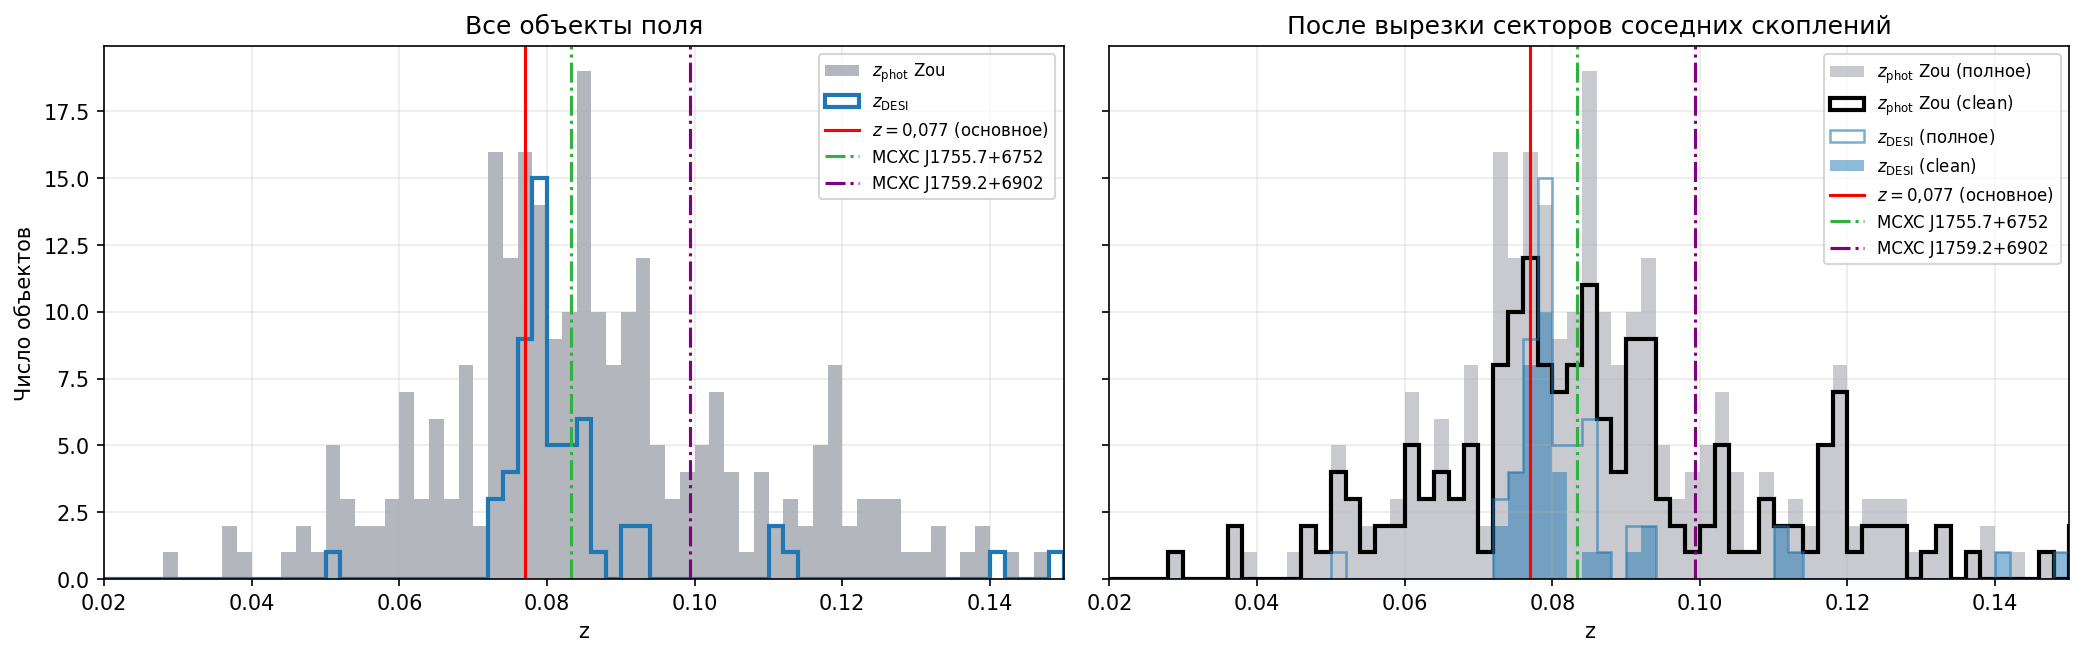
\includegraphics[width=\textwidth]{figures/cluster_zou_histogram.png}
\caption{Распределение объектов поля скопления галактик по красному смещению до (слева) и после (справа) вырезки секторов соседних скоплений. На спектроскопических $z_{\mathrm{DESI}}$ соседние пики исчезают, а на фотометрических $z_{\mathrm{phot}}$ из каталога Zou они сохраняются. Вертикальные линии: $z = 0{,}077$ — основное скопление, $z = 0{,}0833$ — MCXC J1755.7+6752, $z = 0{,}0994$ — MCXC J1759.2+6902.}
\label{fig:cluster-zou}
\end{figure}

В совокупности эти четыре эффекта означают, что разработка моделей фотометрического красного смещения требует не только высокого качества на знакомой выборке, но и явной проверки устойчивости в условиях сдвига распределения, повышенного шума, редких целевых значений и тонкого разрешения близких по $z$ популяций. Именно это определяет дальнейший выбор тестовых наборов и структуру экспериментального стенда.

\subsection{Наборы данных}

В работе рассматриваются два класса наборов данных: табличные фотометрические признаки и многоканальные изображения объектов.

К первому классу относятся Teddy и Happy~\cite{beck2017} с признаками SDSS в фильтрах $u$, $g$, $r$, $i$, $z$, а также SRGz~\cite{meshcheryakov2022} с расширенным набором признаков из нескольких обзоров. Сводные характеристики приведены в таблице~\ref{tab:datasets-summary}.

\begin{table}[H]
\centering
\caption{Сводная характеристика табличных наборов данных}
\label{tab:datasets-summary}
\small
\resizebox{\textwidth}{!}{%
\begin{tabular}{|>{\raggedright\arraybackslash}p{0.22\textwidth}|>{\raggedright\arraybackslash}p{0.24\textwidth}|>{\raggedright\arraybackslash}p{0.24\textwidth}|>{\raggedright\arraybackslash}p{0.24\textwidth}|}
\hline
Характеристика & Teddy & Happy & SRGz \\
\hline
Размер & A — 74\,309, B — 74\,557, C — 97\,980, D — 75\,924 объектов & A — 74\,950, B — 74\,900, C — 60\,315, D — 74\,642 объектов & 411\,696 объектов, из них 304\,291 со спектроскопическим $z$ \\
\hline
Тип объектов & оптические и инфракрасные источники & оптические и инфракрасные источники & рентгеновские источники \\
\hline
Обзор & SDSS & SDSS & SDSS, DESI, Pan-STARRS, DECaLS \\
\hline
Признаки & фотометрические признаки $u$, $g$, $r$, $i$, $z$ & фотометрические признаки $u$, $g$, $r$, $i$, $z$ & рентгеновский поток $F_X$ и отношения $F_X/F_\text{опт}$, оптические магнитуды и цвета SDSS ($u$, $g$, $r$, $i$, $z$), DECaLS ($g$, $r$, $z$) и Pan-STARRS ($g$, $r$, $i$, $z$, $y$), инфракрасные WISE $W1$–$W4$, морфологические индикаторы (Sersic, тип, PSF$-$cmodel) \\
\hline
Пропуски в признаках & отсутствуют & отсутствуют & в компактном наборе из 43 признаков пропуски присутствуют лишь в 84 строках из 411\,696 (менее $0{,}03\%$); в расширенном наборе из 75 признаков около $40\%$ строк содержат хотя бы одно пропущенное значение из-за неполного покрытия SDSS DR16 и Pan-STARRS DR2 \\
\hline
Целевая переменная & фотометрическое красное смещение & фотометрическое красное смещение & фотометрическое красное смещение \\
\hline
Обучающая и тестовая выборки & A — обучающая; B, C, D — тестовые & A — обучающая; B, C, D — тестовые & разбиение в соотношении 80/20 \\
\hline
\end{tabular}
}
\end{table}

Наборы Teddy и Happy содержат по несколько подвыборок: A используется для обучения, B, C и D — как тестовые. Для Teddy это позволяет исследовать устойчивость к сдвигу распределения признаков, для Happy — влияние шума и перенос моделей с ярких объектов на более слабые. Распределения подвыборок вынесены в приложение (рисунки~\ref{fig:teddy-distribution} и~\ref{fig:happy-distribution}): для Teddy подвыборки отличаются формой распределения признаков, для Happy выражен эффект постепенного усложнения данных и роста шума при переходе от B к D.

Набор SRGz включает порядка 300\,000 рентгеновских источников и собирается из нескольких обзоров: СРГ/eROSITA, SDSS DR16, DESI, Pan-STARRS DR2 и DECaLS с привязкой к WISE. Помимо потоков и цветов в нескольких каталогах в него входят межкаталоговые разности магнитуд и морфологические индикаторы (индекс Серсика, тип объекта). В работе используются два варианта признакового описания: компактный набор из 43 признаков с акцентом на DECaLS и WISE и расширенный набор из 75 признаков с добавлением Pan-STARRS и SDSS~DR16.

Второй класс составляют многоканальные изображения объектов. Они содержат фотометрическую и морфологическую информацию. Примеры приведены на рисунке~\ref{fig:galaxy-examples}: для четырех галактик SDSS с разным спектроскопическим $z$ показаны вырезки во всех пяти фильтрах $u$, $g$, $r$, $i$, $z$. Видно, что разные фильтры подсвечивают разные особенности объекта (например, $u$ намного шумнее остальных и плохо передает протяженные структуры), а с ростом $z$ объекты становятся компактнее и слабее на фоне шума.

\begin{figure}[H]
\centering
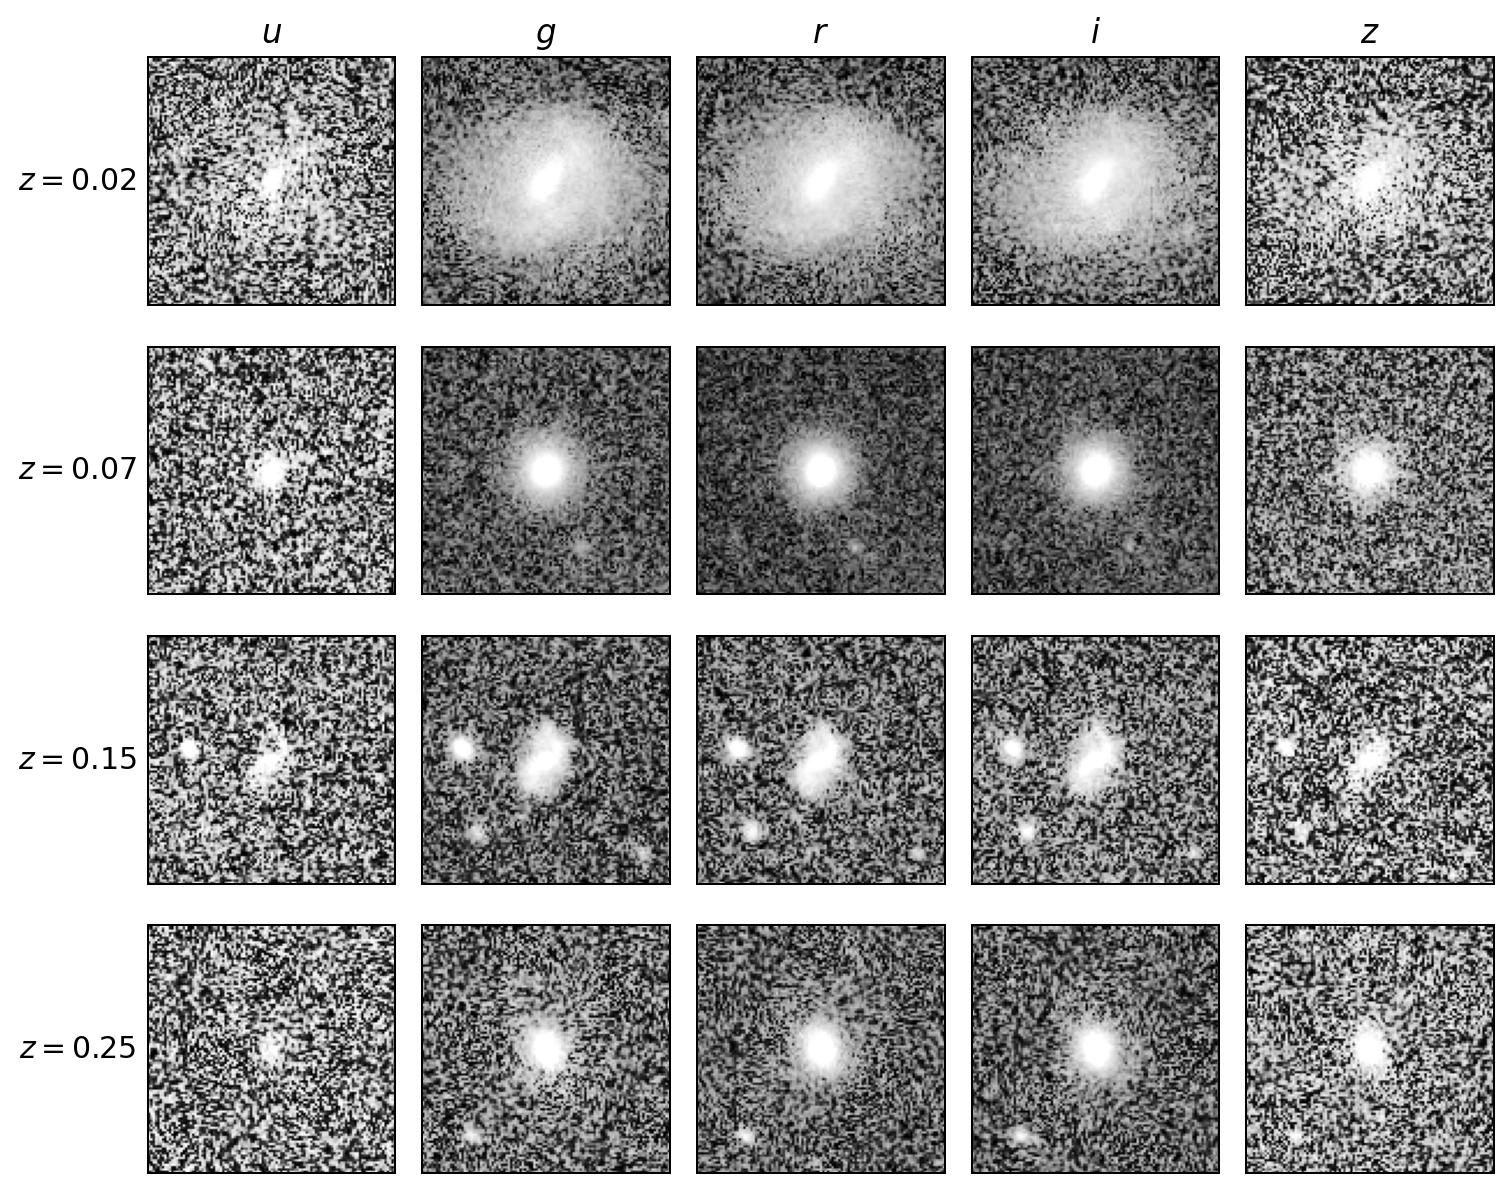
\includegraphics[width=0.85\textwidth]{figures/galaxy_examples.png}
\caption{Примеры изображений галактик из SDSS в пяти фильтрах $u$, $g$, $r$, $i$, $z$. Строки соответствуют разным объектам, упорядоченным по возрастанию спектроскопического красного смещения; столбцы — фильтрам.}
\label{fig:galaxy-examples}
\end{figure}

Для нейросетевых экспериментов используется набор изображений объектов Teddy A/B/C/D, в котором к оптическим фильтрам $g$, $r$, $i$, $z$ добавлены инфракрасные каналы WISE $W1$ и $W2$. Это позволяет вести сравнение моделей на изображениях на тех же объектах, что и сравнение табличных моделей. Сводные характеристики набора приведены в таблице~\ref{tab:image-datasets-summary}.

\begin{table}[H]
\centering
\caption{Характеристика набора изображений Teddy}
\label{tab:image-datasets-summary}
\small
\begin{tabular}{|>{\raggedright\arraybackslash}p{0.30\textwidth}|>{\raggedright\arraybackslash}p{0.60\textwidth}|}
\hline
Размер & A — 74\,098, B — 74\,334, C — 96\,850, D — 75\,722 объектов (более $99\%$ объектов соответствующих табличных подвыборок Teddy) \\
\hline
Источник & вырезки оптических изображений объектов Teddy A/B/C/D, дополненные каналами WISE $W1$ и $W2$ \\
\hline
Размер вырезки & $224 \times 224$ пикселей \\
\hline
Каналы & 6: $g$, $r$, $i$, $z$, $W1$, $W2$ \\
\hline
Формат хранения & один \texttt{.npz}-файл на объект, тензор \texttt{float32} формы $224\!\times\!224\!\times\!6$ \\
\hline
Целевая переменная & фотометрическое красное смещение \\
\hline
Обучающая и тестовая выборки & A — обучающая; B, C, D — тестовые \\
\hline
\end{tabular}
\end{table}

Табличные данные подходят для базового сравнения методов, а изображения дают более полное описание объекта.

\subsection{Алгоритмы классического машинного обучения}

Выбор алгоритмов на табличных признаках строится по принципу покрытия принципиально разных подходов к регрессии, чтобы дальнейшее сравнение разделяло вклад собственно архитектуры модели и вклад типа аппроксимации. Рассматриваются пять методов: CatBoost, Random Forest, многослойный перцептрон, локальная линейная регрессия и обобщенная аддитивная модель (GAM). CatBoost~\cite{dorogush2018catboost} выбран как современный представитель градиентного бустинга над решающими деревьями: бустинг де-факто является базовым ориентиром для табличных задач в фотометрических каталогах и, в частности, использовался в каталоге SRGz~\cite{meshcheryakov2022}. Random Forest~\cite{breiman2001randomforest} включен как классический ансамблевый бейзлайн с независимым построением деревьев: его сравнение с CatBoost позволяет отделить эффект последовательного исправления ошибок от эффекта простого усреднения. Многослойный перцептрон добавлен как нейросетевая модель, строящая гладкое отображение из пространства признаков в красное смещение; именно он использовался как один из основных методов в работе~\cite{beck2017}, в которой и были предложены тесты Teddy и Happy, поэтому включение MLP обеспечивает прямую преемственность с эталонной постановкой и одновременно служит мостом между чисто табличными методами и моделями на изображениях из следующего раздела. Локальная линейная регрессия, исторически широко применявшаяся в задаче фотометрического красного смещения~\cite{beck2017,newman2022}, выбрана как представитель методов окрестностей: она строит предсказание на ближайших объектах и поэтому иначе ведет себя при сдвиге распределения признаков, чем глобальные модели. Наконец, обобщенная аддитивная модель (GAM) добавлена в экспериментальный пайплайн для прямой репликации лучшего табличного бейзлайна из~\cite{beck2017}, где именно этот алгоритм показал наивысшую устойчивость к сдвигу распределения на сложной выборке TeddyD.

\subsubsection{CatBoost}

CatBoost относится к методам градиентного бустинга над решающими деревьями~\cite{dorogush2018catboost}. Модель строит не одно дерево, а последовательность деревьев. Каждое новое дерево обучается исправлять ошибки уже построенного ансамбля. Итоговое предсказание получается как сумма вкладов всех деревьев:
\begin{equation}
\hat{z}(x) = \sum_{m=1}^{M} \eta f_m(x),
\end{equation}
где $f_m(x)$ — очередное дерево, $M$ — число деревьев, $\eta$ — скорость обучения.

Для задачи фотометрического красного смещения CatBoost удобен тем, что работает с табличными признаками и не требует нормализации. Модель делит пространство признаков на области и в каждой области дает свое приближение целевой переменной. Общая схема бустинга приведена на рисунке~\ref{fig:catboost-scheme}.

\begin{figure}[h]
\centering
\resizebox{0.9\textwidth}{!}{%
\begin{tikzpicture}[
    node distance=8mm and 10mm,
    block/.style={draw, rounded corners=2pt, align=center, minimum width=30mm, minimum height=9mm, font=\small},
    arrow/.style={-{Stealth[length=2mm]}, thick, shorten >=1.2mm, shorten <=1.2mm}
]
\node[block] (x) {Фотометрические\\признаки};
\node[block, right=of x] (t1) {Дерево 1\\грубое приближение};
\node[block, right=of t1] (t2) {Дерево 2\\поправка ошибки};
\node[block, right=of t2] (tm) {Дерево $M$\\следующая поправка};
\node[block, right=of tm] (sum) {Сумма\\предсказаний};
\node[block, right=of sum] (out) {$z_{\mathrm{phot}}$};
\draw[arrow] (x) -- (t1);
\draw[arrow] (t1) -- (t2);
\draw[arrow] (t2) -- (tm);
\draw[arrow] (tm) -- (sum);
\draw[arrow] (sum) -- (out);
\end{tikzpicture}
}
\caption{Схема градиентного бустинга в CatBoost.}
\label{fig:catboost-scheme}
\end{figure}

Недостаток бустинга в данной задаче связан с переносом на области признакового пространства, слабо представленные в обучении. Деревья хорошо интерполируют внутри известных областей, но хуже работают при экстраполяции.

\subsubsection{Random Forest}

Random Forest также использует деревья решений, но строит их независимо~\cite{breiman2001randomforest}. Каждое дерево обучается на случайной подвыборке объектов и случайном подмножестве признаков. После этого предсказания деревьев усредняются:
\begin{equation}
\hat{z}(x) = \frac{1}{M}\sum_{m=1}^{M} f_m(x).
\end{equation}

Усреднение снижает дисперсию модели. Если одно дерево переобучилось на случайные особенности выборки, вклад остальных деревьев частично компенсирует эту ошибку. Поэтому случайный лес обычно устойчивее одиночного дерева. Схема работы случайного леса приведена на рисунке~\ref{fig:rf-scheme}.

\begin{figure}[h]
\centering
\resizebox{0.9\textwidth}{!}{%
\begin{tikzpicture}[
    node distance=7mm and 10mm,
    block/.style={draw, rounded corners=2pt, align=center, minimum width=29mm, minimum height=9mm, font=\small},
    arrow/.style={-{Stealth[length=2mm]}, thick}
]
\node[block] (x) {Фотометрические\\признаки};
\node[block, above right=of x] (t1) {Дерево 1};
\node[block, right=of x] (t2) {Дерево 2};
\node[block, below right=of x] (t3) {Дерево $M$};
\node[block, right=35mm of t2] (avg) {Усреднение};
\node[block, right=of avg] (out) {$z_{\mathrm{phot}}$};
\draw[arrow] (x) -- (t1);
\draw[arrow] (x) -- (t2);
\draw[arrow] (x) -- (t3);
\draw[arrow] (t1) -- (avg);
\draw[arrow] (t2) -- (avg);
\draw[arrow] (t3) -- (avg);
\draw[arrow] (avg) -- (out);
\end{tikzpicture}
}
\caption{Схема случайного леса.}
\label{fig:rf-scheme}
\end{figure}

В задаче фотометрического красного смещения Random Forest используется как базовый ансамблевый метод. Его ограничение похоже на ограничение бустинга: дерево выбирает ответ на основе разбиений обучающей выборки, поэтому перенос на другие распределения может быть слабым.

\subsubsection{Многослойный перцептрон}

Многослойный перцептрон является полносвязной нейронной сетью. Он последовательно применяет линейные преобразования и нелинейные функции активации:
\begin{equation}
h_{l+1} = \phi(W_l h_l + b_l),
\end{equation}
где $h_l$ — представление на слое $l$, $W_l$ и $b_l$ — параметры слоя, $\phi$ — нелинейная функция.

В отличие от деревьев, перцептрон строит гладкое отображение из пространства признаков в красное смещение. Поэтому перед обучением признаки нужно нормализовать: разные масштабы признаков ухудшают оптимизацию. Обучение проводится методом обратного распространения ошибки, минимизируя функцию потерь регрессии. Схема многослойного перцептрона приведена на рисунке~\ref{fig:mlp-scheme}.

\begin{figure}[h]
\centering
\resizebox{0.75\textwidth}{!}{%
\begin{tikzpicture}[
    node distance=8mm and 12mm,
    neuron/.style={circle, draw, minimum size=6mm},
    layer/.style={align=center, font=\small},
    arrow/.style={-{Stealth[length=2mm]}, thin}
]
\node[layer] (inlabel) {Признаки};
\node[neuron, below=4mm of inlabel] (i1) {};
\node[neuron, below=of i1] (i2) {};
\node[neuron, below=of i2] (i3) {};

\node[layer, right=25mm of inlabel] (hlabel) {Скрытые\\слои};
\node[neuron, below=4mm of hlabel] (h1) {};
\node[neuron, below=of h1] (h2) {};
\node[neuron, below=of h2] (h3) {};

\node[layer, right=25mm of hlabel] (olabel) {Выход};
\node[neuron, below=12mm of olabel] (o1) {};
\node[right=8mm of o1] (z) {$z_{\mathrm{phot}}$};

\foreach \i in {i1,i2,i3} {
    \foreach \h in {h1,h2,h3} {
        \draw[arrow] (\i) -- (\h);
    }
}
\foreach \h in {h1,h2,h3} {
    \draw[arrow] (\h) -- (o1);
}
\draw[arrow] (o1) -- (z);
\end{tikzpicture}
}
\caption{Схема многослойного перцептрона.}
\label{fig:mlp-scheme}
\end{figure}

В экспериментах MLP важен как модель, не основанная на деревьях. На TeddyD он показывает более низкую долю выбросов, чем CatBoost и Random~Forest, что согласуется с его способностью строить более гладкую зависимость.

\subsubsection{Локальная линейная регрессия}

Локальная линейная регрессия строит предсказание не по всей обучающей выборке сразу, а по окрестности тестового объекта. Для нового объекта сначала выбираются ближайшие соседи в пространстве признаков. Затем на этих соседях обучается линейная модель:
\begin{equation}
\hat{z}(x) = \beta_0 + \sum_{j=1}^{p}\beta_j x_j.
\end{equation}

Такой подход использует предположение о локальной гладкости: близкие объекты в пространстве фотометрических признаков должны иметь близкие красные смещения. В отличие от глобальной линейной регрессии, коэффициенты модели подбираются отдельно для каждой окрестности. Схема локальной аппроксимации приведена на рисунке~\ref{fig:llr-scheme}.

\begin{figure}[h]
\centering
\resizebox{0.9\textwidth}{!}{%
\begin{tikzpicture}[
    node distance=8mm and 10mm,
    block/.style={draw, rounded corners=2pt, align=center, minimum width=31mm, minimum height=9mm, font=\small},
    arrow/.style={-{Stealth[length=2mm]}, thick}
]
\node[block] (x) {Новый объект};
\node[block, right=of x] (neighbors) {Поиск ближайших\\соседей};
\node[block, right=of neighbors] (local) {Линейная модель\\на соседях};
\node[block, right=of local] (out) {$z_{\mathrm{phot}}$};
\draw[arrow] (x) -- (neighbors);
\draw[arrow] (neighbors) -- (local);
\draw[arrow] (local) -- (out);
\end{tikzpicture}
}
\caption{Схема локальной линейной регрессии.}
\label{fig:llr-scheme}
\end{figure}

В задаче Teddy этот метод оказывается устойчивым при переносе на TeddyD по $\sigma_{NMAD}$. Это можно объяснить тем, что локальная аппроксимация меньше зависит от глобальной формы распределения обучающей выборки.

\subsubsection{Обобщенная аддитивная модель (GAM)}

Обобщенная аддитивная модель (Generalized Additive Model, GAM) представляет собой развитие линейной регрессии, в которой влияние каждого признака моделируется с помощью нелинейных гладких функций. В задаче регрессии красного смещения модель имеет вид:
\begin{equation}
\hat{z}(x) = \beta_0 + \sum_{j=1}^{p} f_j(x_j),
\end{equation}
где $f_j$ — нелинейные функции (чаще всего сглаживающие сплайны), подбираемые в процессе обучения. Использование сплайнов позволяет модели выучивать сложные нелинейные зависимости между отдельным признаком (например, звездной величиной или цветом) и целевой переменной. В то же время аддитивная структура сохраняет интерпретируемость: вклад каждого признака можно проанализировать независимо от остальных.

В контексте задачи фотометрического красного смещения GAM обладает важным свойством — способностью к контролируемой экстраполяции. Благодаря штрафам за кривизну сплайнов (регуляризации) вне области обучающих данных модель ведет себя как линейная. Это объясняет высокую устойчивость GAM на сдвинутых выборках (таких как TeddyD), где метод продемонстрировал лучшие результаты среди эмпирических алгоритмов в эталонном исследовании Beck~et~al.~\cite{beck2017}.

\subsection{Подходы глубокого обучения}

Архитектуры для работы с изображениями выбраны так, чтобы охватить три магистральные ветви развития компьютерного зрения и одну специализированную линию, связанную напрямую с задачей фотометрического красного смещения. Базовый ориентир задает EfficientNet~\cite{tan2019efficientnet} — современная сверточная сеть с согласованным масштабированием глубины, ширины и разрешения, удобная как опорная точка благодаря умеренному размеру и широкой воспроизводимости результатов. ConvNeXt~\cite{liu2022convnext} включен как обновленный сверточный дизайн, в котором архитектура CNN переосмыслена с учетом приемов трансформеров и на стандартных задачах распознавания достигает качества чисто трансформерных моделей; это позволяет проверить, дает ли возврат к свертке преимущество в условиях ограниченного и шумного астрономического входа. Vision Transformer~\cite{dosovitskiy2020vit} добавлен как представитель чисто трансформерной ветви: он проверяет, переносится ли преимущество трансформеров с задач ImageNet на изображения галактик, в которых сцена существенно беднее, а полезный сигнал сосредоточен в центре кадра. CapsNet рассматривается отдельно: капсульная архитектура была предложена для photoz в работе~\cite{dey2022} как способ совместить регрессию красного смещения с распознаванием морфологии и получить более интерпретируемое представление объекта, поэтому ее включение в обзор позволяет оценить, переносится ли заявленное в~\cite{dey2022} преимущество капсул на бенчмарк Teddy. Таким образом, четыре выбранные архитектуры представляют свертку, гибрид свертки и трансформера, чистый трансформер и капсульный подход — каждая из них отвечает на отдельный исследовательский вопрос о том, какой класс моделей лучше подходит для photoz по изображениям.

\subsubsection{EfficientNet}

EfficientNet представляет собой семейство сверточных сетей с согласованным масштабированием глубины, ширины и входного разрешения~\cite{tan2019efficientnet}. Обычная сверточная сеть извлекает признаки последовательно: ранние слои выделяют локальные структуры, а более глубокие слои строят более абстрактное представление изображения. EfficientNet сохраняет эту схему, но масштабирует архитектуру не по одному параметру, а сразу по трем: числу слоев, числу каналов и разрешению входа.

Для задачи фотометрического красного смещения EfficientNet используется как базовая модель на изображениях. На вход подаются изображения объекта в нескольких фильтрах. Первая свертка адаптируется к числу входных каналов, после чего сеть извлекает визуальные признаки. Последний классификационный слой заменяется регрессионной головой, которая выдает одно число: оценку красного смещения. Общая схема приведена на рисунке~\ref{fig:efficientnet-scheme}.

\begin{figure}[h]
\centering
\resizebox{0.9\textwidth}{!}{%
\begin{tikzpicture}[
    node distance=8mm and 11mm,
    block/.style={draw, rounded corners=2pt, align=center, minimum width=28mm, minimum height=9mm, font=\small},
    arrow/.style={-{Stealth[length=2mm]}, thick}
]
\node[block] (input) {Изображение\\в нескольких фильтрах};
\node[block, right=of input] (stem) {Начальная\\свертка};
\node[block, right=of stem] (blocks) {Сверточные\\блоки EfficientNet};
\node[block, right=of blocks] (pool) {Глобальное\\усреднение};
\node[block, right=of pool] (head) {Регрессионная\\голова};
\node[block, right=of head] (out) {$z_{\mathrm{phot}}$};
\draw[arrow] (input) -- (stem);
\draw[arrow] (stem) -- (blocks);
\draw[arrow] (blocks) -- (pool);
\draw[arrow] (pool) -- (head);
\draw[arrow] (head) -- (out);
\end{tikzpicture}
}
\caption{Схема применения EfficientNet к оценке фотометрического красного смещения.}
\label{fig:efficientnet-scheme}
\end{figure}

Преимущество EfficientNet состоит в том, что это компактная сверточная модель с готовыми предварительно обученными весами. Поэтому ее удобно использовать как отправную точку для сравнения с более сложными архитектурами.

\subsubsection{ConvNeXt}

ConvNeXt является сверточной архитектурой, которая была спроектирована как современная версия сверточной сети~\cite{liu2022convnext}. Она сохраняет основную идею сверточной обработки изображения, но использует ряд решений, характерных для более поздних архитектур: крупные ядра глубинных сверток, нормализацию по каналам, блочную структуру и более простую схему нелинейностей.

На практике ConvNeXt работает как иерархический извлекатель признаков. Изображение сначала переводится в набор признаковых карт, затем разрешение постепенно уменьшается, а число каналов растет. Благодаря этому сеть одновременно учитывает локальные детали и более крупные структуры изображения. Для астрономических объектов это полезно: модель может учитывать как центральную яркость, так и распределение света вокруг объекта. Базовая схема такой обработки приведена на рисунке~\ref{fig:convnext-scheme}.

\begin{figure}[h]
\centering
\resizebox{0.9\textwidth}{!}{%
\begin{tikzpicture}[
    node distance=8mm and 10mm,
    block/.style={draw, rounded corners=2pt, align=center, minimum width=28mm, minimum height=9mm, font=\small},
    arrow/.style={-{Stealth[length=2mm]}, thick}
]
\node[block] (input) {Изображение};
\node[block, right=of input] (patch) {Начальное\\разбиение};
\node[block, right=of patch] (s1) {Стадия 1\\высокое разрешение};
\node[block, right=of s1] (s2) {Стадии 2–4\\меньше разрешение\\больше каналов};
\node[block, right=of s2] (head) {Усреднение\\и регрессия};
\node[block, right=of head] (out) {$z_{\mathrm{phot}}$};
\draw[arrow] (input) -- (patch);
\draw[arrow] (patch) -- (s1);
\draw[arrow] (s1) -- (s2);
\draw[arrow] (s2) -- (head);
\draw[arrow] (head) -- (out);
\end{tikzpicture}
}
\caption{Схема ConvNeXt как иерархической сверточной модели.}
\label{fig:convnext-scheme}
\end{figure}

В данной работе ConvNeXt-Tiny уже показал лучший результат среди рассмотренных моделей на изображениях на подвыборке TeddyD. Поэтому эта архитектура рассматривается не только как обзорный вариант, но и как один из основных кандидатов для дальнейших экспериментов.

\subsubsection{Vision Transformer}

Vision Transformer переносит идею Transformer на изображения~\cite{dosovitskiy2020vit}. Вместо последовательности слов модель получает последовательность фрагментов изображения. Каждый фрагмент переводится в вектор, к нему добавляется информация о положении, после чего последовательность обрабатывается кодировщиком Transformer.

Главное отличие от сверточных сетей состоит в способе учета контекста. Свертка сначала работает локально, а более широкий контекст появляется после нескольких слоев. В Transformer каждый фрагмент может напрямую учитывать другие фрагменты через механизм внимания. Это полезно, если информация о красном смещении связана не только с локальными деталями, но и с распределением яркости по всему изображению. Схема применения Vision Transformer приведена на рисунке~\ref{fig:vit-scheme}.

\begin{figure}[h]
\centering
\resizebox{0.9\textwidth}{!}{%
\begin{tikzpicture}[
    node distance=8mm and 10mm,
    block/.style={draw, rounded corners=2pt, align=center, minimum width=28mm, minimum height=9mm, font=\small},
    arrow/.style={-{Stealth[length=2mm]}, thick}
]
\node[block] (input) {Изображение};
\node[block, right=of input] (patches) {Фрагменты\\изображения};
\node[block, right=of patches] (embed) {Векторные\\представления};
\node[block, right=of embed] (encoder) {Кодировщик\\Transformer};
\node[block, right=of encoder] (head) {Регрессионная\\голова};
\node[block, right=of head] (out) {$z_{\mathrm{phot}}$};
\draw[arrow] (input) -- (patches);
\draw[arrow] (patches) -- (embed);
\draw[arrow] (embed) -- (encoder);
\draw[arrow] (encoder) -- (head);
\draw[arrow] (head) -- (out);
\end{tikzpicture}
}
\caption{Схема Vision Transformer для регрессии красного смещения.}
\label{fig:vit-scheme}
\end{figure}

Недостаток такого подхода состоит в том, что Transformer обычно требует больше данных для устойчивого обучения. Поэтому в экспериментах ViT-Tiny используется как компактная версия архитектуры.

\subsubsection{CapsNet}

CapsNet отличается от обычных сверточных сетей тем, что передает между слоями не скалярные активации, а векторы. Длина такого вектора интерпретируется как вероятность класса, а направление кодирует свойства объекта на изображении. Для галактик это удобно: ориентация, размер, вытянутость и распределение яркости несут информацию о морфологии и могут быть связаны с красным смещением.

В работе Dey и соавторов~\cite{dey2022} капсульная архитектура применяется к изображениям SDSS в пяти фильтрах $u$, $g$, $r$, $i$, $z$ размером $64 \times 64$ пикселя. В отличие от исходной CapsNet~\cite{sabour2017capsnet}, авторы используют вариант DeepCaps~\cite{rajasegaran2019deepcaps} с остаточными капсульными блоками: это позволяет применять капсульный подход к относительно глубокой сети без квадратичного роста числа параметров от полного routing-а на каждом уровне. Архитектура состоит из трех частей: капсульного энкодера, декодера-регуляризатора и регрессора красного смещения. Схема приведена на рисунке~\ref{fig:capsnet-scheme}.

\begin{figure}[h]
\centering
\resizebox{\textwidth}{!}{%
\begin{tikzpicture}[
    node distance=6mm and 8mm,
    block/.style={
        draw,
        rounded corners=2pt,
        align=center,
        minimum width=30mm,
        minimum height=9mm,
        font=\small
    },
    smallblock/.style={
        draw,
        rounded corners=2pt,
        align=center,
        minimum width=27mm,
        minimum height=8mm,
        font=\small
    },
    arrow/.style={-{Stealth[length=2mm]}, thick}
]
\node[block] (input) {Изображение\\$64\times64\times5$};
\node[block, right=of input] (stem) {Conv $128$, $3{\times}3$\\BatchNorm};
\node[block, right=of stem] (blocks) {4 остаточных\\капсульных блока\\(DeepCaps)};
\node[block, right=of blocks] (digit) {Финальный\\routing\\$2$ капсулы $\times\,16$};
\node[smallblock, above right=of digit] (decoder) {Декодер\\$5$ ConvTranspose};
\node[smallblock, below right=of digit] (regressor) {Регрессор\\$128{-}64{-}32{-}16{-}1$};
\node[smallblock, right=of decoder] (recon) {Восстановленное\\изображение};
\node[smallblock, right=of regressor] (zphot) {$z_{\mathrm{phot}}$};

\draw[arrow] (input) -- (stem);
\draw[arrow] (stem) -- (blocks);
\draw[arrow] (blocks) -- (digit);
\draw[arrow] (digit) -- (decoder);
\draw[arrow] (digit) -- (regressor);
\draw[arrow] (decoder) -- (recon);
\draw[arrow] (regressor) -- (zphot);
\end{tikzpicture}
}
\caption{Схема CapsNet для оценки фотометрического красного смещения по изображениям. После сверточного стема и четырех остаточных капсульных блоков финальный routing формирует две капсулы (спиральная / эллиптическая), которые подаются в декодер-регуляризатор и регрессор красного смещения.}
\label{fig:capsnet-scheme}
\end{figure}

Энкодер начинается с обычной свертки $128$ ядер $3 \times 3$ с активацией ReLU и нормализацией по батчу, после чего изображение интерпретируется как набор $128$ капсул размерности $1$. Далее идут четыре остаточных капсульных блока. Внутри каждого блока понижающий капсульный слой со страйдом $2$ уменьшает пространственное разрешение, после чего три капсульных слоя без понижения разрешения формируют остаточную ветвь, складываемую с пропускным соединением. Все слои внутри блока выполняют локальную свертку капсульных активаций без полного механизма маршрутизации; такая упрощенная локальная маршрутизация эквивалентна сверточному преобразованию с последующей нелинейностью squash и сохраняет векторную природу капсул при существенно меньших затратах. Полная маршрутизация применяется в двух местах: на пропускном соединении последнего блока (трехмерный капсульный сверточный слой с тремя итерациями routing-а) и в финальном слое, где двухуровневая капсульная карта объединяется и преобразуется в две капсулы размерности $16$.

Длина каждой из двух итоговых капсул используется как оценка вероятности соответствующего морфологического класса (спиральная или эллиптическая галактика). Во время обучения в декодер и регрессор подается капсула правильного класса (по метке Galaxy Zoo-1), а во время применения модели — капсула с наибольшей длиной.

Декодер восстанавливает исходное изображение по выбранной капсуле и работает как регуляризатор: капсула должна хранить достаточно информации, чтобы по ней можно было восстановить форму, ориентацию и распределение яркости галактики. В реализации авторов декодер состоит из полносвязного слоя, разворачивающего капсулу размерности $16$ в тензор $5 \times 64 \times 64$, и пяти последовательных слоев транспонированной свертки $3 \times 3$ с активациями PReLU и финальным $\tanh$. Регрессор получает ту же капсулу и через четыре полносвязных слоя $128 \to 64 \to 32 \to 16$ с активациями PReLU предсказывает фотометрическое красное смещение в логистически преобразованной шкале.

Логистическое преобразование переводит ограниченный диапазон $z \in [z_{\min}, z_{\max}]$ ($z_{\min} = 0$, $z_{\max} = 0.4$) в неограниченный диапазон, в котором удобнее обучать регрессионную голову на основе средней квадратичной ошибки:
\begin{equation}
y = \log\frac{z - z_{\min}}{z_{\max} - z}, \qquad
z = \frac{e^{y}\, z_{\max} + z_{\min}}{e^{y} + 1}.
\end{equation}

Обучение в статье проходит в два этапа. Сначала авторы обучают капсульный классификатор морфологии вместе с декодером на объектах с надежными метками Galaxy Zoo-1. После этого модель используется для разметки объектов без таких меток, и затем обучается полная сеть, включая регрессор красного смещения. Итоговая функция потерь объединяет три члена:
\begin{equation}
L = L_{\mathrm{margin}} + \alpha L_{\mathrm{decoder}} + \beta L_z, \quad
\alpha = 0.005,\ \beta = 1.
\end{equation}

Здесь $L_{\mathrm{margin}}$ отвечает за морфологическую классификацию~\cite{sabour2017capsnet}:
\begin{equation}
L_{\mathrm{margin}} =
\sum_{j=1}^{2}
T_j \max(0, m^+ - \lVert v_j \rVert)^2
+ \lambda (1 - T_j)\max(0, \lVert v_j \rVert - m^-)^2,
\end{equation}
где $v_j$ — капсула класса $j$, $T_j$ — индикатор правильного класса, $m^+=0.9$, $m^-=0.1$, $\lambda=0.5$. Эта часть функции потерь увеличивает длину капсулы правильного класса и уменьшает длину капсулы неправильного класса.

Потеря декодера — средняя квадратичная разность между исходным и восстановленным изображениями (для согласованности с активацией $\tanh$ декодера значения пикселей предварительно делятся на масштабный множитель):
\begin{equation}
L_{\mathrm{decoder}} =
\frac{1}{5 \cdot 64 \cdot 64}\sum_{k=1}^{5}\sum_{p=1}^{64}\sum_{q=1}^{64}
(x_{pqk} - \hat{x}_{pqk})^2.
\end{equation}
Для регрессии используется квадратичная ошибка в логистически преобразованной шкале:
\begin{equation}
L_z = (y_{\mathrm{spec}} - y_{\mathrm{phot}})^2,\qquad
y = \log\frac{z - z_{\min}}{z_{\max} - z}.
\end{equation}

Таким образом, модель одновременно решает три задачи: определяет морфологический тип, кодирует изображение в капсулу и предсказывает фотометрическое красное смещение. Это отличает ее от обычной сверточной сети, где внутреннее представление обычно труднее интерпретировать.

Рабочая гипотеза состоит в том, что классические алгоритмы дают базовый уровень на табличных признаках, а модели на изображениях могут быть устойчивее к сдвигу распределения, шуму и смещению к среднему.

\subsection{Метрики качества}

Поскольку задача фотометрического красного смещения является задачей регрессии, одной средней ошибки недостаточно. В астрономической литературе широко применяются специализированные метрики, позволяющие оценивать как типичную точность, так и долю крупных промахов.

Для оценки качества используются следующие показатели:
\begin{itemize}
    \item доля катастрофических выбросов;
    \item нормализованное медианное абсолютное отклонение (NMAD);
    \item систематическое смещение.
\end{itemize}

Пусть $z_{\mathrm{gt},i}$ и $z_{\mathrm{pred},i}$ — истинное и предсказанное красное смещение $i$-го объекта, $N$ — размер выборки. Введём нормализованную ошибку предсказания:
\[
\Delta z_i = \frac{z_{\mathrm{pred},i} - z_{\mathrm{gt},i}}{1 + z_{\mathrm{gt},i}}.
\]
Тогда используемые метрики записываются следующим образом:
\begin{align}
\mathrm{bias} &= \mathrm{median}(\Delta z_i), \\
\sigma_{\mathrm{NMAD}} &= 1{,}48 \cdot \mathrm{median}\!\left(|\Delta z_i - \mathrm{bias}|\right), \\
f_{\mathrm{outlier}} &= \frac{1}{N}\sum_{i=1}^{N} \mathbf{1}\!\left[|\Delta z_i| \ge 0{,}15\right].
\end{align}

Здесь $\sigma_{\mathrm{NMAD}}$ характеризует типичный масштаб ошибки, $\mathrm{bias}$ отражает систематическое смещение предсказаний, а $f_{\mathrm{outlier}}$ — доля объектов, для которых нормализованная ошибка превышает порог $0{,}15$.

Этот набор метрик позволяет учитывать типичную ошибку, bias и долю грубых промахов.

\subsection{Выводы по обзору}

По результатам обзора можно сделать несколько выводов. Во-первых, табличные модели необходимы как бейзлайн, поскольку они сравнительно просты, быстро обучаются и позволяют надежно воспроизводить эксперименты. Во-вторых, именно на тестах Teddy и Happy проявляются ограничения таких моделей: они чувствительны к изменению распределения и уровню шума. В-третьих, архитектуры глубокого обучения на изображениях представляют практический интерес не только из-за более высокой выразительной способности, но и потому, что они могут использовать морфологическую информацию объекта. Поэтому дальнейшее исследование в работе строится как последовательное сравнение табличных и визуальных подходов в едином экспериментальном стенде.

\newpage
\section{Исследование и решение задачи}

Логика исследования в работе строится как последовательность этапов. Сначала требуется создать экспериментальный стенд, позволяющий единообразно запускать эксперименты на разных выборках и моделях. Затем необходимо исследовать поведение выбранных алгоритмов на наборах Teddy, Happy и SRGz. После этого можно переходить к обобщению результатов и к формулировке направлений дальнейшего развития метода.

Такой порядок обусловлен не только техническими, но и методическими соображениями. Без воспроизводимого стенда трудно сравнивать модели между собой и отделять влияние архитектуры от влияния случайных параметров запуска. Кроме того, задача фотометрического красного смещения чувствительна к распределению данных, поэтому результаты на одном наборе еще не позволяют делать общие выводы. Поэтому в исследовании используются несколько сценариев: тест на экстраполяцию (Teddy), тест на устойчивость к шуму (Happy) и прикладной каталог рентгеновских источников (SRGz).

На первом этапе рассматриваются классические модели для табличных признаков. Они дают воспроизводимый бейзлайн и позволяют проверить основные гипотезы о трудности задачи.

\subsection{Декомпозиция задачи и обоснование решений}

Для достижения цели работы исходная задача была разложена на следующие подзадачи:
\begin{enumerate}[label=\arabic*.]
    \item проанализировать существующие подходы к оценке фотометрического красного смещения и на этой основе выбрать наборы данных, алгоритмы и метрики качества;
    \item разработать экспериментальный стенд для воспроизводимого запуска моделей, сохранения артефактов и формирования отчётов;
    \item исследовать поведение выбранных моделей на наборах Teddy, Happy и SRGz;
    \item сравнить классические табличные алгоритмы с нейросетевыми подходами, использующими изображения;
    \item сформулировать выводы о применимости рассматриваемых методов и направлениях дальнейшего развития.
\end{enumerate}

Выбор наборов данных, алгоритмов и метрик обоснован в разделе~\ref{sec:review} (обзор литературы). Ключевое решение, не вытекающее из обзора напрямую, — построение собственного экспериментального стенда вместо адаптации готового инструмента. Задача одновременно требует поддержки двух принципиально разных форматов входных данных: табличных файлов с фотометрическими признаками и каталогов изображений в формате \texttt{npz}. Готовые фреймворки ориентированы, как правило, на один из этих форматов, и унификация метрик, отчётов и артефактов потребовала бы сопоставимого объёма доработки. Собственный стенд позволяет контролировать каждый шаг пайплайна и добавлять новые модели или сплиты без изменения остальных компонентов. Его архитектура описана в разделе~\ref{sec:experiment}.

\newpage
\section{Практическая часть, эксперимент}
\label{sec:experiment}

\subsection{Экспериментальный стенд}

Необходимость отдельного экспериментального стенда вытекает из самой постановки задачи фотометрического красного смещения. В работе сравниваются заметно разнородные модели — от градиентного бустинга на табличных признаках до сверточных и капсульных сетей на многоканальных изображениях — на нескольких независимых тестовых сплитах: Teddy A$\to$B/C/D, Happy A$\to$B/C/D и SRGz. Исследовательский вывод формируется не одним числом, а совокупностью метрик, оцениваемых на разных сценариях деградации распределения, поэтому полное число запусков измеряется десятками. В таком режиме попытка вести эксперименты в формате отдельных скриптов или интерактивных нотбуков быстро приводит к потере связи между метрикой и условиями, в которых она получена: какая версия кода работала, какие параметры были выставлены, к какому именно сплиту относится результат. Это формирует первое требование — прозрачность экспериментирования.

К этому добавляется специфика оценки качества: основной интерес представляет не точность на знакомой выборке, а характер деградации при переходе на тестовые сплиты, в том числе со сдвигом распределения. В таком режиме результат чувствителен к мелким деталям предобработки, инициализации весов и порядка обработки данных, поэтому ценность эксперимента критически зависит от того, можно ли точно повторить запуск через месяцы и понять, какие именно изменения объясняют сдвиг метрик между двумя версиями модели. Не менее важно, что эксперимент должен быть повторяем не только автором: научный руководитель, рецензент или сторонний исследователь, имея исходный код, конфигурацию и данные, должны получить те же численные результаты независимо от среды и истории работы автора. Отсюда вытекает требование воспроизводимости. Параллельно исследование заведомо предполагает подключение новых алгоритмов и наборов признаков по мере появления гипотез, а часть выводов получается не по одному запуску, а по сводным таблицам, объединяющим несколько моделей на нескольких сплитах. Это требует расширяемости и единых процедур расчета метрик: без них сравнения оказываются технически несопоставимыми, а интерпретация различий — спорной.

Наконец, объем экспериментов и характерное время обучения нейросетевых моделей делают невыгодным полный пересчет пайплайна при изменении одного шага: смена признаков для табличной модели не должна обесценивать ранее посчитанные нейросетевые предсказания, а независимые запуски естественно ускоряются при наличии нескольких GPU и ядер CPU. Из этого вытекает четвертое требование — эффективные вычисления. Альтернативные акценты, например удобство интерактивной работы или богатство визуализации, рассматриваются как полезные, но вторичные: они улучшают исследовательский опыт, но не закрывают перечисленных рисков потери информации, несопоставимости результатов и непосильного объема пересчета. Поэтому в основу стенда положены именно четыре ключевых требования:
\begin{itemize}
    \item прозрачность экспериментирования;
    \item воспроизводимость;
    \item расширяемость;
    \item эффективные вычисления.
\end{itemize}

Под прозрачностью понимается возможность по сохраненным результатам однозначно восстановить, какие данные использовались, какие параметры были заданы, какой вариант исходного кода запускался и какие процедуры привели к полученным метрикам. Воспроизводимость означает, что один и тот же эксперимент на тех же данных, с теми же исходными текстами и параметрами должен приводить к тем же численным результатам. Расширяемость требуется для поддержки новых алгоритмов, новых наборов признаков и, в более общем случае, разных постановок задачи: регрессии и классификации. Эффективные вычисления важны потому, что экспериментальный стенд должен уметь пересчитывать только изменившиеся части вычислительного процесса и управлять параллельностью запуска отдельных этапов.

На практике эти требования реализуются через несколько взаимосвязанных компонентов экспериментального процесса:
\begin{enumerate}[label=\arabic*.]
    \item описание данных и сплитов, где фиксируются входные каталоги, форматы хранения и правила разбиения выборок;
    \item библиотека методов, где реализуются модели, метрики, преобразования данных и вспомогательные алгоритмы;
    \item вычислительный процесс, который последовательно выполняет подготовку данных, обучение, получение предсказаний и расчет метрик;
    \item компонент артефактов и отчетности, где сохраняются параметры запуска, обученные модели, предсказания, метрики, графики и сравнительные таблицы.
\end{enumerate}

Такая организация позволяет запускать эксперимент как единый воспроизводимый процесс. Подготовка данных, обучение, получение предсказаний, расчет метрик и формирование отчетов выполняются по общей конфигурации, а промежуточные и итоговые результаты сохраняются как артефакты запуска.

\subsection{Конфигурация стенда в репозитории}

Структура репозитория отражает разделение стенда на библиотечные модули, сценарии запуска, конфигурации и артефакты экспериментов. В библиотечных модулях реализованы загрузка данных, метрики, обучение табличных моделей, локальная линейная регрессия и вспомогательные функции. Нейросетевые компоненты выделены отдельно: в них находятся загрузчик изображений, утилиты обучения и реализация CapsNet. Сценарии запуска задают входные точки для подготовки данных, обучения, применения моделей, расчета метрик и генерации отчетов.

Оркестрация эксперимента выполняется с помощью Prefect. В стенде Prefect отвечает за управление вычислительным процессом: он объединяет отдельные этапы в единый поток выполнения, задает порядок их выполнения и явно фиксирует зависимости между подготовкой данных, обучением, применением моделей, расчетом метрик и построением отчетов. Благодаря этому полный эксперимент запускается как единая процедура, а не как набор ручных команд.

Конфигурация верхнего уровня определяет, какая ветка вычислительного процесса должна быть выполнена: табличная или нейросетевая. Для табличных моделей оркестратор сначала подготавливает данные и затем последовательно запускает обучение, получение предсказаний и расчет метрик для каждой модели из конфигурации. Для нейросетевых моделей подготовка табличного сплита не требуется: обучение выполняется по изображениям, после чего сохраненная модель применяется к заданным тестовым сплитам. В обоих случаях итоговые предсказания приводятся к общему формату, поэтому расчет метрик и сводная отчетность остаются одинаковыми.

\subsection{Архитектура программного средства}

Архитектура стенда сводится к одному повторяемому потоку: конфигурация задает данные, модель и выходные каталоги; вычислительный процесс выполняет подготовку данных, обучение, получение предсказаний, расчет метрик и выпуск отчетов. Различие между табличными моделями и нейросетями скрыто внутри отдельных шагов, но итоговый формат результатов остается общим. На рисунке~\ref{fig:repo-architecture} приведена базовая схема стенда: она фиксирует основную последовательность этапов и связь между входными данными, конфигурациями, моделью, предсказаниями, метриками и отчетом.

\begin{figure}[H]
\centering
\includegraphics[width=\textwidth]{figures/stand_scheme_presentation.png}
\caption{Базовая схема экспериментального стенда.}
\label{fig:repo-architecture}
\end{figure}

Отдельно формируется сводный отчет по нескольким запускам. Схема этого процесса приведена на рисунке~\ref{fig:summary-report-scheme}.

\begin{figure}[H]
\centering
\includegraphics[width=0.9\textwidth]{figures/stand_summary_scheme.png}
\caption{Схема формирования сводного отчета по нескольким экспериментам.}
\label{fig:summary-report-scheme}
\end{figure}

Центральным элементом является оркестратор эксперимента. Для табличных моделей он запускает подготовку каталога признаков, обучение модели, получение предсказаний и расчет метрик. Для нейросетей подготовленный табличный сплит не используется: модель обучается по изображениям и каталогу истинных красных смещений, после чего сохраняется лучшая версия модели. После получения предсказаний обе ветки сходятся к одному формату таблицы, поэтому метрики и отчеты строятся одинаково. После каждого запуска стенд сохраняет конфигурацию, описание сплита, обученную модель, таблицу предсказаний и диагностические материалы — набор, достаточный для воспроизведения и анализа результата.

\subsection{Результаты}

Сводные результаты экспериментов приведены в таблице~\ref{tab:all-results}. В ней оставлены только профильные метрики задачи фотометрического красного смещения: $\sigma_{NMAD}$, доля выбросов и bias. Все численные значения получены в актуальной версии стенда: табличные модели обучены на подвыборках Teddy A и Happy A соответственно и применены ко всем тестовым сплитам B, C, D; модели на изображениях обучены на Teddy A.

\begin{table}[htbp]
\centering
\caption{Сводные результаты по всем подвыборкам и алгоритмам. В каждой подвыборке жирным выделен лучший по $\sigma_{NMAD}$ метод.}
\label{tab:all-results}
\small
\begin{tabular}{|l|l|c|c|c|}
\hline
Подвыборка & Модель & $\sigma_{NMAD}$ & $f_{\mathrm{outlier}}, \%$ & bias $(10^{-2})$ \\
\hline
\multirow{8}{*}{TeddyB} & \textbf{CatBoost} & \textbf{0.0170} & \textbf{0.18} & \textbf{0.014} \\
 & LLR & 0.0171 & 0.18 & 0.041 \\
 & MLP & 0.0171 & 0.16 & -0.003 \\
 & RF & 0.0174 & 0.18 & 0.034 \\
 & GAM & 0.0199 & 0.10 & 0.026 \\
 & EfficientNet-B0 & 0.0204 & 0.12 & -0.641 \\
 & ConvNeXt-Tiny & 0.0228 & 0.51 & -0.516 \\
 & ViT-Tiny & 0.0413 & 1.12 & 2.121 \\
\hline
\multirow{8}{*}{TeddyC} & \textbf{CatBoost} & \textbf{0.0170} & 0.27 & -0.016 \\
 & \textbf{LLR} & \textbf{0.0170} & 0.26 & 0.004 \\
 & \textbf{MLP} & \textbf{0.0170} & \textbf{0.25} & \textbf{-0.039} \\
 & RF & 0.0174 & 0.26 & 0.016 \\
 & GAM & 0.0205 & 0.17 & 0.062 \\
 & EfficientNet-B0 & 0.0209 & 0.17 & -0.531 \\
 & ConvNeXt-Tiny & 0.0236 & 0.59 & -0.511 \\
 & ViT-Tiny & 0.0408 & 1.12 & 2.071 \\
\hline
\multirow{8}{*}{TeddyD} & CatBoost & 0.0764 & 8.14 & -0.059 \\
 & LLR & 0.0360 & 3.71 & 1.559 \\
 & MLP & 0.0395 & 3.23 & 2.110 \\
 & RF & 0.0790 & 6.00 & -0.192 \\
 & \textbf{GAM} & \textbf{0.0329} & \textbf{2.16} & \textbf{-0.014} \\
 & EfficientNet-B0 & 0.0662 & 4.35 & -0.569 \\
 & ConvNeXt-Tiny & 0.0346 & 2.35 & -1.373 \\
 & ViT-Tiny & 0.0483 & 5.39 & 1.369 \\
\hline
\multirow{5}{*}{HappyB} & \textbf{CatBoost} & \textbf{0.0207} & \textbf{1.01} & \textbf{0.082} \\
 & LLR & 0.0208 & 1.14 & 0.168 \\
 & MLP & 0.0213 & 0.97 & 0.332 \\
 & RF & 0.0228 & 1.07 & 0.176 \\
 & GAM & 0.0328 & 1.63 & 0.196 \\
\hline
\multirow{5}{*}{HappyC} & \textbf{CatBoost} & \textbf{0.0515} & \textbf{5.86} & \textbf{0.349} \\
 & LLR & 0.0554 & 6.50 & 0.723 \\
 & MLP & 0.0529 & 5.85 & 0.615 \\
 & RF & 0.0553 & 5.77 & 0.713 \\
 & GAM & 0.0758 & 11.61 & 3.391 \\
\hline
\multirow{5}{*}{HappyD} & \textbf{CatBoost} & \textbf{0.0810} & 15.21 & -0.331 \\
 & LLR & 0.0839 & 14.53 & -0.561 \\
 & \textbf{MLP} & \textbf{0.0810} & \textbf{14.36} & \textbf{-0.065} \\
 & RF & 0.0823 & 14.12 & -0.556 \\
 & GAM & 0.1062 & 18.86 & -0.115 \\
\hline
\end{tabular}
\end{table}

Из таблицы~\ref{tab:all-results} видно, что на TeddyB и TeddyC классические модели работают близко по всем основным метрикам ($\sigma_{NMAD} \approx 0{,}017$). На TeddyD картина меняется кардинально: CatBoost и Random~Forest деградируют наиболее резко ($\sigma_{NMAD} = 0{,}076$ и $0{,}079$ соответственно), тогда как GAM оказывается наиболее устойчивым среди табличных методов ($\sigma_{NMAD} = 0{,}033$, $f_{\mathrm{outlier}} = 2{,}16\%$), демонстрируя способность к экстраполяции за пределы обучающего распределения. LLR и MLP занимают промежуточное положение ($\sigma_{NMAD} = 0{,}036$ и $0{,}040$).

Для прямого сравнения в таблице~\ref{tab:beck2017-baselines} приведены базовые результаты эмпирических методов из~\cite{beck2017} на тех же подвыборках. Полученные в данной работе значения $\sigma_{NMAD}$ для LLR и Random~Forest на TeddyB/C совпадают с эталонными в пределах $\sim 0{,}001$, что подтверждает корректность реализации стенда. На наиболее сложной подвыборке TeddyD лучшим по~\cite{beck2017} оказывается GAM — глобальный непараметрический метод, способный экстраполировать за пределы признакового пространства обучения ($\sigma_{NMAD}=0{,}033$, $f_\mathrm{outlier}=2{,}28\%$). В нашей реализации сопоставимые результаты на TeddyD дает ConvNeXt-Tiny ($\sigma_{NMAD}=0{,}035$, $f_\mathrm{outlier}=2{,}35\%$), что показывает, что на этом сплите модель на изображениях вплотную приближается к уровню лучшего табличного метода (GAM). На HappyD по~\cite{beck2017} различие между эмпирическими методами невелико: лучший результат у Random~Forest ($\sigma_{NMAD}=0{,}079$), что согласуется с поведением наших табличных моделей на этом сплите.

\begin{table}[htbp]
\centering
\caption{Базовые результаты эмпирических методов из~\cite{beck2017} на подвыборках Teddy и Happy. Значения $\sigma_{NMAD}$ получены пересчетом приведенных в~\cite{beck2017} значений MAD по соотношению $\sigma_{NMAD} = 1{,}48 \cdot \mathrm{MAD}$. Лучший по $\sigma_{NMAD}$ метод на TeddyD и HappyD выделен жирным.}
\label{tab:beck2017-baselines}
\small
\begin{tabular}{|l|l|c|c|c|}
\hline
Подвыборка & Модель & $\sigma_{NMAD}$ & $f_{\mathrm{outlier}}, \%$ & bias $(10^{-2})$ \\
\hline
\multirow{4}{*}{TeddyB} & ANNz & 0.0172 & 0.18 & 0.03 \\
 & GAM & 0.0198 & 0.11 & 0.05 \\
 & LLR & 0.0169 & 0.19 & 0.07 \\
 & RF & 0.0175 & 0.17 & 0.03 \\
\hline
\multirow{4}{*}{TeddyC} & ANNz & 0.0170 & 0.26 & -0.01 \\
 & GAM & 0.0204 & 0.18 & 0.06 \\
 & LLR & 0.0169 & 0.28 & 0.05 \\
 & RF & 0.0173 & 0.26 & -0.01 \\
\hline
\multirow{4}{*}{TeddyD} & ANNz & 0.0534 & 3.09 & -0.08 \\
 & \textbf{GAM} & \textbf{0.0330} & \textbf{2.28} & \textbf{-0.06} \\
 & LLR & 0.0364 & 3.80 & 1.76 \\
 & RF & 0.0775 & 6.70 & 0.16 \\
\hline
\multirow{4}{*}{HappyB} & ANNz & 0.0221 & 0.99 & 0.04 \\
 & GAM & 0.0289 & 1.36 & 0.09 \\
 & LLR & 0.0206 & 1.11 & 0.13 \\
 & RF & 0.0209 & 1.02 & 0.05 \\
\hline
\multirow{4}{*}{HappyC} & ANNz & 0.0533 & 5.59 & 0.16 \\
 & GAM & 0.0716 & 7.37 & 0.86 \\
 & LLR & 0.0531 & 6.07 & 0.52 \\
 & RF & 0.0519 & 5.58 & 0.34 \\
\hline
\multirow{4}{*}{HappyD} & ANNz & 0.0805 & 14.01 & -0.52 \\
 & GAM & 0.0992 & 16.38 & -0.51 \\
 & LLR & 0.0832 & 14.52 & -0.79 \\
 & \textbf{RF} & \textbf{0.0793} & \textbf{14.20} & \textbf{-0.28} \\
\hline
\end{tabular}
\end{table}

На наборе Happy характер деградации иной. CatBoost остаётся лучшим или одним из лучших на HappyB и HappyC, на HappyD CatBoost и MLP делят первое место ($\sigma_{\mathrm{NMAD}} = 0{,}081$); при этом все модели деградируют значительно: у CatBoost, MLP, LLR и RF $\sigma_{\mathrm{NMAD}}$ вырастает с $\approx 0{,}021$ на HappyB до $\approx 0{,}081$ на HappyD; у GAM — с $0{,}033$ до $0{,}106$. GAM на протяжении всей последовательности B→D уступает остальным, в том числе демонстрируя наибольшую долю выбросов ($f_{\mathrm{outlier}} = 18{,}86\%$ на HappyD). Это подтверждает, что фотометрический шум и смещение по яркости являются тяжёлым фактором для всех классических табличных методов без исключения, а не только для отдельных архитектур.

Отдельный табличный эксперимент был проведен на каталоге SRGz. Набор соответствует прикладной задаче для рентгеновских источников и включает признаки из нескольких оптических и инфракрасных обзоров. Результаты приведены в таблице~\ref{tab:srgz-fast-results}. На текущем этапе для SRGz доступны только табличные признаки: набор изображений для этого каталога пока не подготовлен.

\begin{table}[htbp]
\centering
\caption{Результаты табличного эксперимента на SRGz. Лучший по $\sigma_{NMAD}$ метод выделен жирным.}
\label{tab:srgz-fast-results}
\small
\begin{tabular}{|l|c|c|c|}
\hline
Модель & $\sigma_{NMAD}$ & $f_{\mathrm{outlier}}, \%$ & bias $(10^{-2})$ \\
\hline
CatBoost & 0.0797 & 15.50 & 0.463 \\
LLR & 0.0801 & 17.19 & 1.063 \\
\textbf{MLP} & \textbf{0.0773} & \textbf{14.17} & \textbf{-0.109} \\
Random Forest & 0.0919 & 19.13 & 0.999 \\
GAM & 0.1304 & 28.47 & 1.019 \\
\hline
\end{tabular}
\end{table}

\begin{figure}[H]
\centering
\begin{subfigure}{0.32\textwidth}\centering\includegraphics[width=\linewidth]{figures/scatters/srgz_catboost.png}\caption{CatBoost}\end{subfigure}\hfill
\begin{subfigure}{0.32\textwidth}\centering\includegraphics[width=\linewidth]{figures/scatters/srgz_mlp.png}\caption{MLP}\end{subfigure}\hfill
\begin{subfigure}{0.32\textwidth}\centering\includegraphics[width=\linewidth]{figures/scatters/srgz_llr.png}\caption{LLR}\end{subfigure}

\vspace{0.4em}
\begin{subfigure}{0.32\textwidth}\centering\includegraphics[width=\linewidth]{figures/scatters/srgz_rf.png}\caption{Random Forest}\end{subfigure}\hfill
\begin{subfigure}{0.32\textwidth}\centering\includegraphics[width=\linewidth]{figures/scatters/srgz_gam.png}\caption{GAM}\end{subfigure}\hfill
\begin{subfigure}{0.32\textwidth}\phantom{x}\end{subfigure}
\caption{Диаграммы рассеяния предсказаний на каталоге SRGz.}
\label{fig:scatter-srgz}
\end{figure}

На SRGz все классические модели дают заметно более высокие значения $\sigma_{NMAD}$ и доли выбросов, чем на простых подвыборках TeddyB/TeddyC. Лучший результат показывает MLP ($\sigma_{NMAD}=0{,}0773$, $f_{\mathrm{outlier}}=14{,}17\%$), близко к нему находится CatBoost. Random~Forest и особенно GAM оказываются слабее. Локальная линейная регрессия имеет близкое к CatBoost значение робастной метрики, однако отдельные экстремальные предсказания делают этот метод менее устойчивым в прикладном смысле. В совокупности результаты подтверждают, что для SRGz классических табличных алгоритмов недостаточно: на качество одновременно влияют сдвиг распределения, шум наблюдений, неоднородность источников и смещение предсказаний к основной массе обучающей выборки.

Калибровочные кривые SRGz приведены на рисунке~\ref{fig:calib-srgz}. Все модели хорошо следуют диагонали в диапазоне $z \lesssim 1{,}5$, однако при $z > 2$ наблюдается выраженное уплощение: ни одна из моделей не достигает истинных значений красного смещения выше~$\approx 2{,}1$. Это наглядно демонстрирует attenuation bias на реальном прикладном каталоге.

\begin{figure}[H]
\centering
\includegraphics[width=0.55\textwidth]{figures/scatters/srgz_calibration.png}
\caption{Калибровочные кривые для всех табличных моделей на каталоге SRGz. Ломаные показывают медианное предсказанное $z$ в равновероятностных бинах по истинному~$z$.}
\label{fig:calib-srgz}
\end{figure}

Среди представленных в таблице моделей на изображениях наиболее сильные результаты на сложной подвыборке TeddyD показывает ConvNeXt-Tiny ($\sigma_{NMAD}=0{,}0346$). Опорная сверточная модель EfficientNet-B0 демонстрирует хорошую точность на базовых наборах TeddyB и TeddyC ($\sigma_{NMAD} \approx 0{,}020$), однако на TeddyD ее ошибка возрастает почти в три раза ($\sigma_{NMAD}=0{,}0662$), что говорит о меньшей устойчивости классической свертки к сильному сдвигу распределения по сравнению с иерархической архитектурой ConvNeXt. Архитектура Vision Transformer (ViT-Tiny), напротив, показывает слабые результаты на простых выборках ($\sigma_{NMAD} \approx 0{,}041$), но демонстрирует удивительную стабильность при переходе к TeddyD, где ее ошибка возрастает незначительно ($\sigma_{NMAD}=0{,}0483$). Это подтверждает гипотезу о том, что трансформеры обладают высокой обобщающей способностью, но требуют большего объема данных для достижения базового уровня качества сверточных сетей. Кроме того, по сравнению с табличными моделями (CatBoost, RF) ухудшение качества при переходе к TeddyD для ConvNeXt и ViT оказывается менее резким. Это поддерживает целесообразность перехода к обучению на изображениях в условиях сдвига.

Для визуального сравнения качества предсказаний на каждой подвыборке на рисунках~\ref{fig:scatter-teddyB}–\ref{fig:scatter-happyD} приведены диаграммы рассеяния в осях «истинное значение — предсказанное значение» для всех моделей. Для табличных моделей строится по одному графику на каждый сплит; для моделей на изображениях — только на подвыборках Teddy, где они обучены и применены. На графиках видно, что в простом режиме (TeddyB, TeddyC, HappyB) предсказания всех табличных моделей плотно сконцентрированы вдоль диагонали, тогда как при экстраполяции (TeddyD) и при росте шума (HappyC, HappyD) разброс существенно увеличивается, особенно у CatBoost и Random~Forest. Среди моделей на изображениях ConvNeXt-Tiny демонстрирует наименьший визуальный разброс на TeddyD, что согласуется с метриками таблицы~\ref{tab:all-results}.

\begin{figure}[H]
\centering
\begin{subfigure}{0.245\textwidth}\centering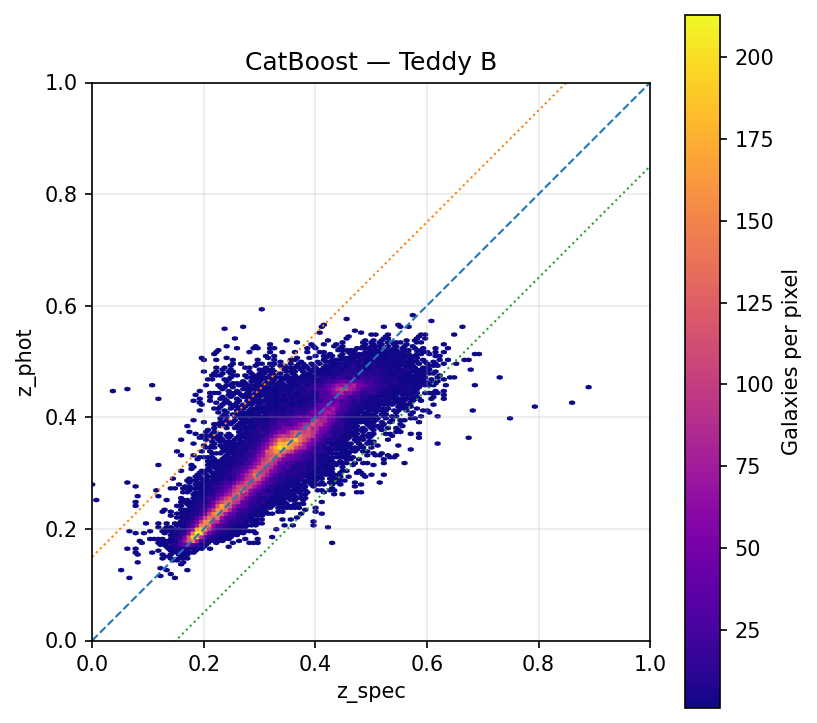
\includegraphics[width=\linewidth]{figures/scatters/catboost_teddy_B.png}\caption{CatBoost}\end{subfigure}\hfill
\begin{subfigure}{0.245\textwidth}\centering\includegraphics[width=\linewidth]{figures/scatters/rf_teddy_B.png}\caption{Random Forest}\end{subfigure}\hfill
\begin{subfigure}{0.245\textwidth}\centering\includegraphics[width=\linewidth]{figures/scatters/mlp_teddy_B.png}\caption{MLP}\end{subfigure}\hfill
\begin{subfigure}{0.245\textwidth}\centering\includegraphics[width=\linewidth]{figures/scatters/llr_teddy_B.png}\caption{LLR}\end{subfigure}

\vspace{0.4em}
\begin{subfigure}{0.245\textwidth}\centering\includegraphics[width=\linewidth]{figures/scatters/gam_teddy_B.png}\caption{GAM}\end{subfigure}\hfill
\begin{subfigure}{0.245\textwidth}\centering\includegraphics[width=\linewidth]{figures/scatters/efficientnet_teddy_B.png}\caption{EfficientNet-B0}\end{subfigure}\hfill
\begin{subfigure}{0.245\textwidth}\centering\includegraphics[width=\linewidth]{figures/scatters/convnext_teddy_B.png}\caption{ConvNeXt-Tiny}\end{subfigure}\hfill
\begin{subfigure}{0.245\textwidth}\centering\includegraphics[width=\linewidth]{figures/scatters/vit_teddy_B.png}\caption{ViT-Tiny}\end{subfigure}
\caption{Диаграммы рассеяния предсказаний на TeddyB.}
\label{fig:scatter-teddyB}
\end{figure}

\begin{figure}[H]
\centering
\begin{subfigure}{0.245\textwidth}\centering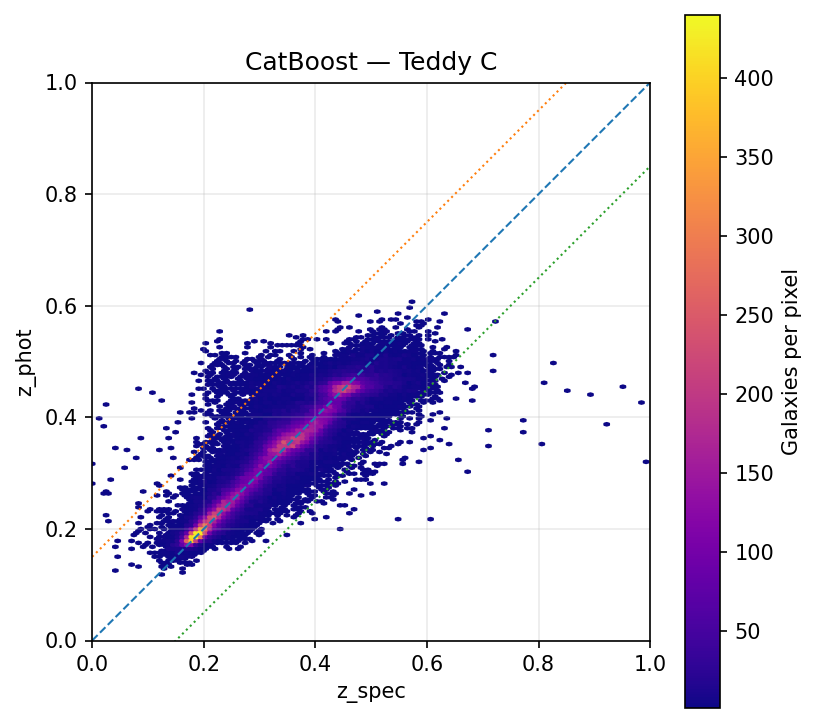
\includegraphics[width=\linewidth]{figures/scatters/catboost_teddy_C.png}\caption{CatBoost}\end{subfigure}\hfill
\begin{subfigure}{0.245\textwidth}\centering\includegraphics[width=\linewidth]{figures/scatters/rf_teddy_C.png}\caption{Random Forest}\end{subfigure}\hfill
\begin{subfigure}{0.245\textwidth}\centering\includegraphics[width=\linewidth]{figures/scatters/mlp_teddy_C.png}\caption{MLP}\end{subfigure}\hfill
\begin{subfigure}{0.245\textwidth}\centering\includegraphics[width=\linewidth]{figures/scatters/llr_teddy_C.png}\caption{LLR}\end{subfigure}

\vspace{0.4em}
\begin{subfigure}{0.245\textwidth}\centering\includegraphics[width=\linewidth]{figures/scatters/gam_teddy_C.png}\caption{GAM}\end{subfigure}\hfill
\begin{subfigure}{0.245\textwidth}\centering\includegraphics[width=\linewidth]{figures/scatters/efficientnet_teddy_C.png}\caption{EfficientNet-B0}\end{subfigure}\hfill
\begin{subfigure}{0.245\textwidth}\centering\includegraphics[width=\linewidth]{figures/scatters/convnext_teddy_C.png}\caption{ConvNeXt-Tiny}\end{subfigure}\hfill
\begin{subfigure}{0.245\textwidth}\centering\includegraphics[width=\linewidth]{figures/scatters/vit_teddy_C.png}\caption{ViT-Tiny}\end{subfigure}
\caption{Диаграммы рассеяния предсказаний на TeddyC.}
\label{fig:scatter-teddyC}
\end{figure}

\begin{figure}[H]
\centering
\begin{subfigure}{0.245\textwidth}\centering\includegraphics[width=\linewidth]{figures/scatters/catboost_teddy_D.png}\caption{CatBoost}\end{subfigure}\hfill
\begin{subfigure}{0.245\textwidth}\centering\includegraphics[width=\linewidth]{figures/scatters/rf_teddy_D.png}\caption{Random Forest}\end{subfigure}\hfill
\begin{subfigure}{0.245\textwidth}\centering\includegraphics[width=\linewidth]{figures/scatters/mlp_teddy_D.png}\caption{MLP}\end{subfigure}\hfill
\begin{subfigure}{0.245\textwidth}\centering\includegraphics[width=\linewidth]{figures/scatters/llr_teddy_D.png}\caption{LLR}\end{subfigure}

\vspace{0.4em}
\begin{subfigure}{0.245\textwidth}\centering\includegraphics[width=\linewidth]{figures/scatters/gam_teddy_D.png}\caption{GAM}\end{subfigure}\hfill
\begin{subfigure}{0.245\textwidth}\centering\includegraphics[width=\linewidth]{figures/scatters/efficientnet_teddy_D.png}\caption{EfficientNet-B0}\end{subfigure}\hfill
\begin{subfigure}{0.245\textwidth}\centering\includegraphics[width=\linewidth]{figures/scatters/convnext_teddy_D.png}\caption{ConvNeXt-Tiny}\end{subfigure}\hfill
\begin{subfigure}{0.245\textwidth}\centering\includegraphics[width=\linewidth]{figures/scatters/vit_teddy_D.png}\caption{ViT-Tiny}\end{subfigure}
\caption{Диаграммы рассеяния предсказаний на TeddyD.}
\label{fig:scatter-teddyD}
\end{figure}

\begin{figure}[H]
\centering
\begin{subfigure}{0.32\textwidth}\centering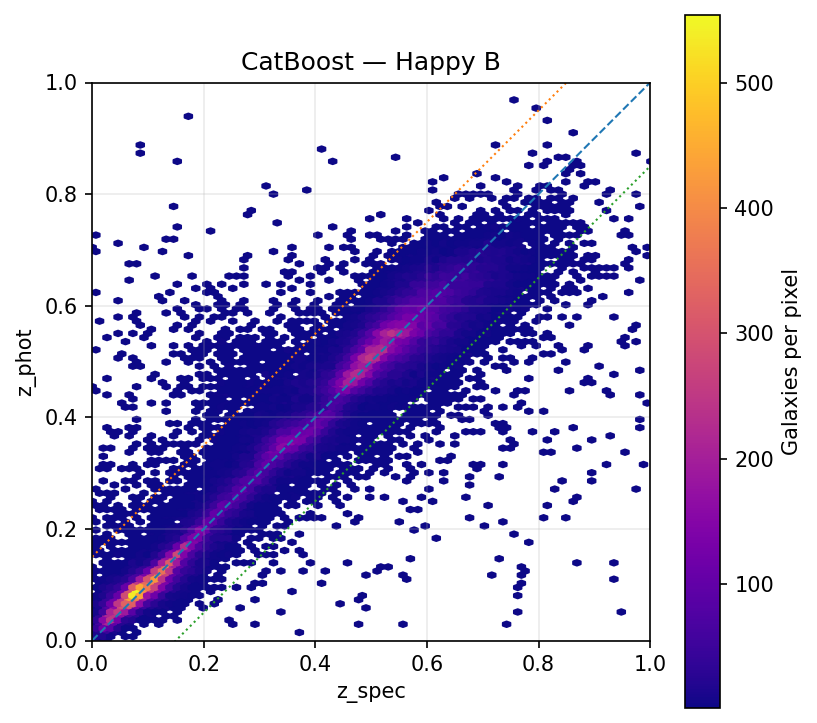
\includegraphics[width=\linewidth]{figures/scatters/catboost_happy_B.png}\caption{CatBoost}\end{subfigure}\hfill
\begin{subfigure}{0.32\textwidth}\centering\includegraphics[width=\linewidth]{figures/scatters/rf_happy_B.png}\caption{Random Forest}\end{subfigure}\hfill
\begin{subfigure}{0.32\textwidth}\centering\includegraphics[width=\linewidth]{figures/scatters/mlp_happy_B.png}\caption{MLP}\end{subfigure}

\vspace{0.4em}
\begin{subfigure}{0.32\textwidth}\centering\includegraphics[width=\linewidth]{figures/scatters/llr_happy_B.png}\caption{LLR}\end{subfigure}\hfill
\begin{subfigure}{0.32\textwidth}\centering\includegraphics[width=\linewidth]{figures/scatters/gam_happy_B.png}\caption{GAM}\end{subfigure}\hfill
\begin{subfigure}{0.32\textwidth}\centering~\end{subfigure}
\caption{Диаграммы рассеяния предсказаний на HappyB.}
\label{fig:scatter-happyB}
\end{figure}

\begin{figure}[H]
\centering
\begin{subfigure}{0.32\textwidth}\centering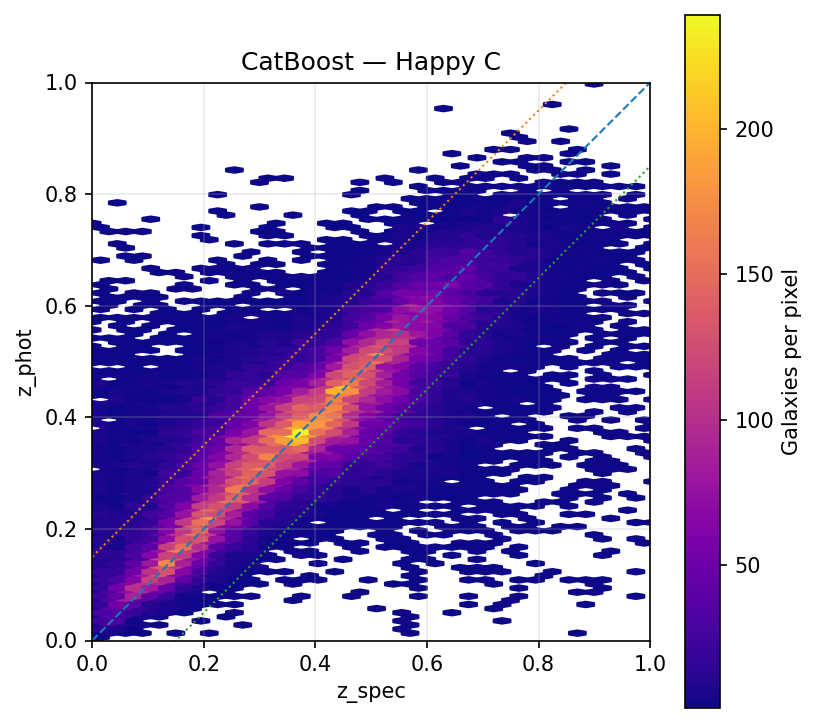
\includegraphics[width=\linewidth]{figures/scatters/catboost_happy_C.png}\caption{CatBoost}\end{subfigure}\hfill
\begin{subfigure}{0.32\textwidth}\centering\includegraphics[width=\linewidth]{figures/scatters/rf_happy_C.png}\caption{Random Forest}\end{subfigure}\hfill
\begin{subfigure}{0.32\textwidth}\centering\includegraphics[width=\linewidth]{figures/scatters/mlp_happy_C.png}\caption{MLP}\end{subfigure}

\vspace{0.4em}
\begin{subfigure}{0.32\textwidth}\centering\includegraphics[width=\linewidth]{figures/scatters/llr_happy_C.png}\caption{LLR}\end{subfigure}\hfill
\begin{subfigure}{0.32\textwidth}\centering\includegraphics[width=\linewidth]{figures/scatters/gam_happy_C.png}\caption{GAM}\end{subfigure}\hfill
\begin{subfigure}{0.32\textwidth}\centering~\end{subfigure}
\caption{Диаграммы рассеяния предсказаний на HappyC.}
\label{fig:scatter-happyC}
\end{figure}

\begin{figure}[H]
\centering
\begin{subfigure}{0.32\textwidth}\centering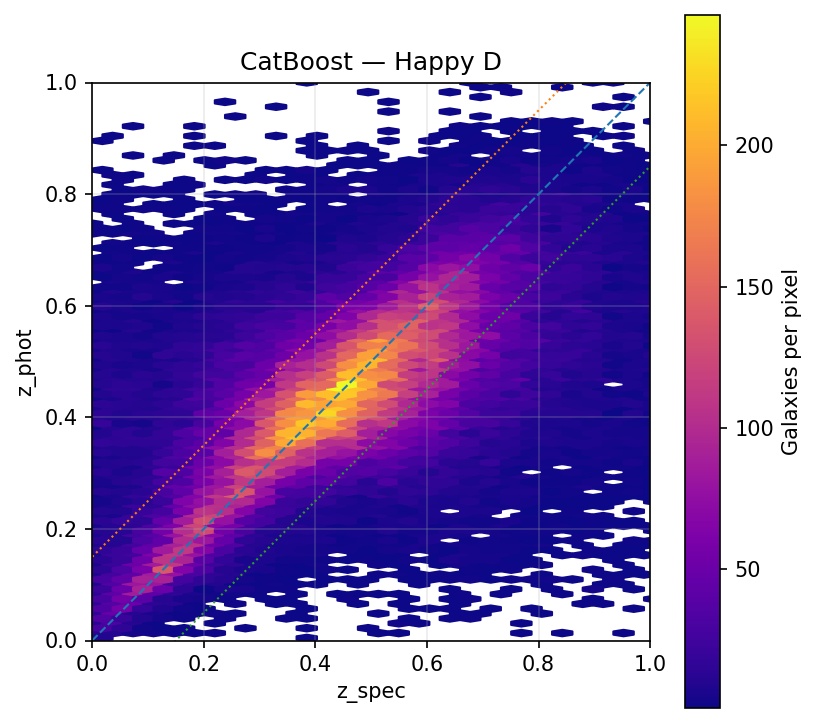
\includegraphics[width=\linewidth]{figures/scatters/catboost_happy_D.png}\caption{CatBoost}\end{subfigure}\hfill
\begin{subfigure}{0.32\textwidth}\centering\includegraphics[width=\linewidth]{figures/scatters/rf_happy_D.png}\caption{Random Forest}\end{subfigure}\hfill
\begin{subfigure}{0.32\textwidth}\centering\includegraphics[width=\linewidth]{figures/scatters/mlp_happy_D.png}\caption{MLP}\end{subfigure}

\vspace{0.4em}
\begin{subfigure}{0.32\textwidth}\centering\includegraphics[width=\linewidth]{figures/scatters/llr_happy_D.png}\caption{LLR}\end{subfigure}\hfill
\begin{subfigure}{0.32\textwidth}\centering\includegraphics[width=\linewidth]{figures/scatters/gam_happy_D.png}\caption{GAM}\end{subfigure}\hfill
\begin{subfigure}{0.32\textwidth}\centering~\end{subfigure}
\caption{Диаграммы рассеяния предсказаний на HappyD.}
\label{fig:scatter-happyD}
\end{figure}

Помимо диаграмм рассеяния, систематические ошибки модели удобно оценивать по \emph{калибровочным графикам}: истинное красное смещение разбивается на $15$ квантильных бинов, в каждом бине вычисляется среднее истинное значение и среднее предсказанное значение, а затем строится зависимость одного среднего от другого. У идеально откалиброванной модели полученная ломаная совпадает с диагональю $y=x$; систематический недостаток или избыток предсказания в определенной области $z$ проявляется как соответствующее отклонение от диагонали. На рисунках~\ref{fig:calib-teddyB}–\ref{fig:calib-happyD} приведены такие графики для всех подвыборок; на одних осях изображены все модели, что позволяет напрямую сопоставлять характер их систематических смещений.

\begin{figure}[H]
\centering
\begin{subfigure}{0.32\textwidth}\centering
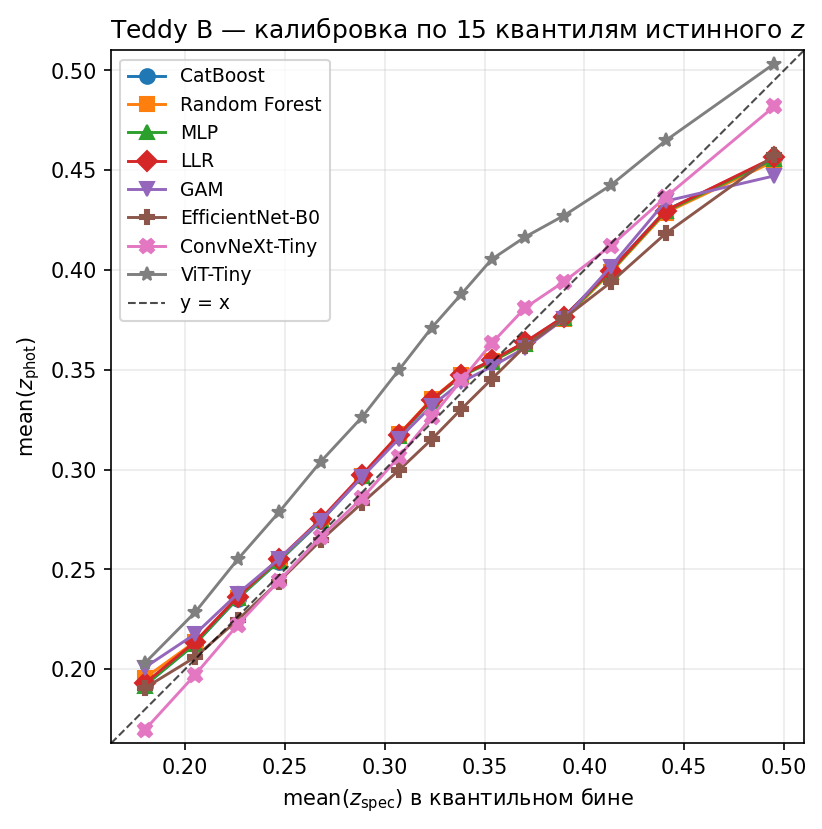
\includegraphics[width=\linewidth]{figures/calibration/calibration_teddy_B.png}
\caption{TeddyB}\label{fig:calib-teddyB}
\end{subfigure}\hfill
\begin{subfigure}{0.32\textwidth}\centering
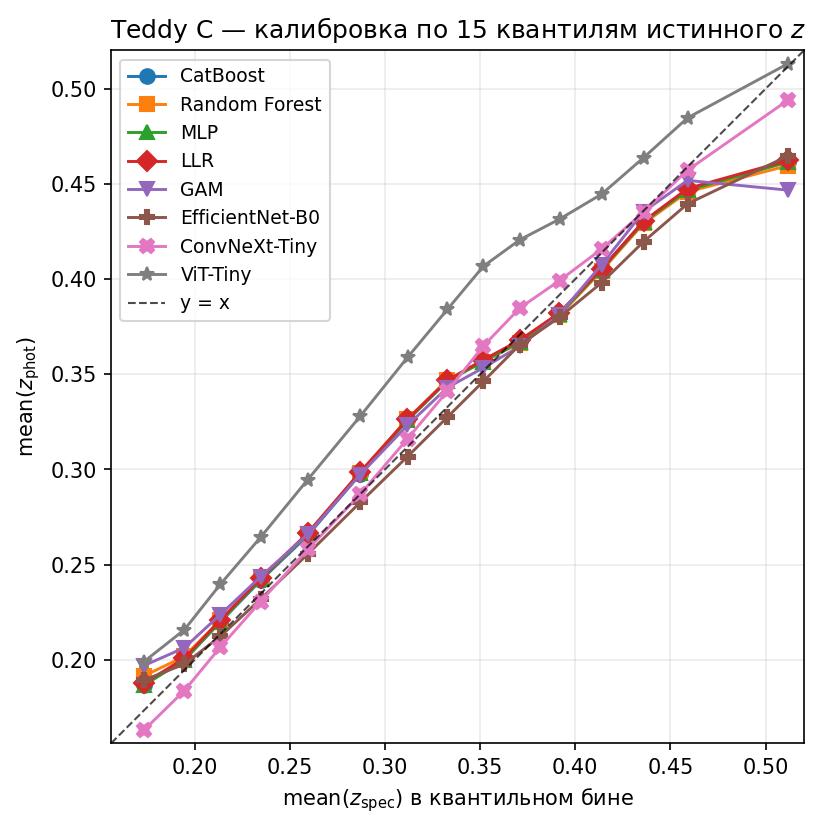
\includegraphics[width=\linewidth]{figures/calibration/calibration_teddy_C.png}
\caption{TeddyC}\label{fig:calib-teddyC}
\end{subfigure}\hfill
\begin{subfigure}{0.32\textwidth}\centering
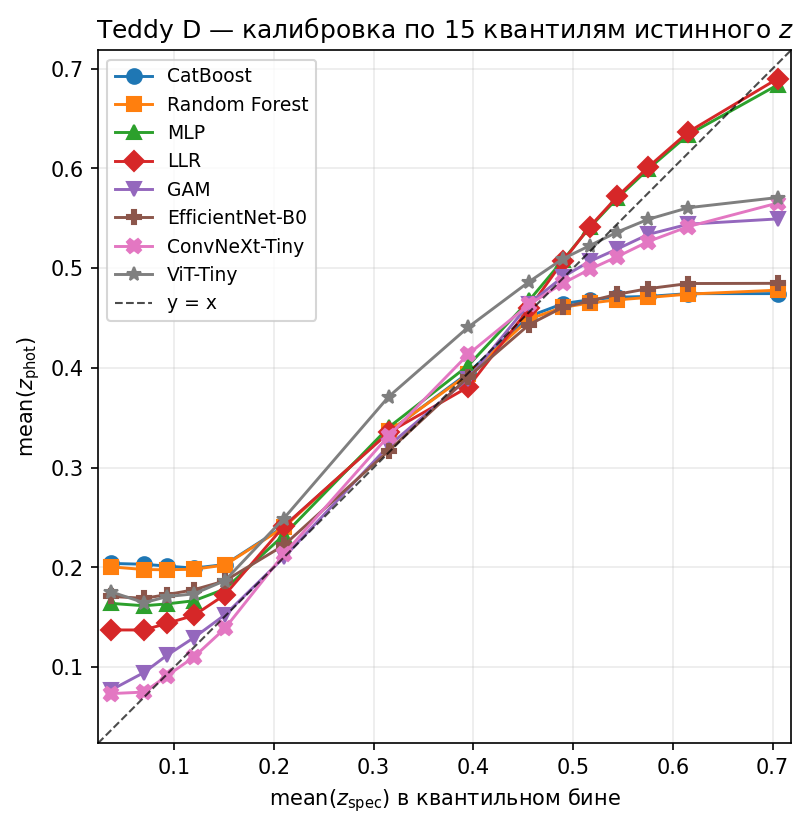
\includegraphics[width=\linewidth]{figures/calibration/calibration_teddy_D.png}
\caption{TeddyD}\label{fig:calib-teddyD}
\end{subfigure}
\caption{Калибровочные кривые на подвыборках Teddy.}
\label{fig:calib-teddy}
\end{figure}

\begin{figure}[H]
\centering
\begin{subfigure}{0.32\textwidth}\centering
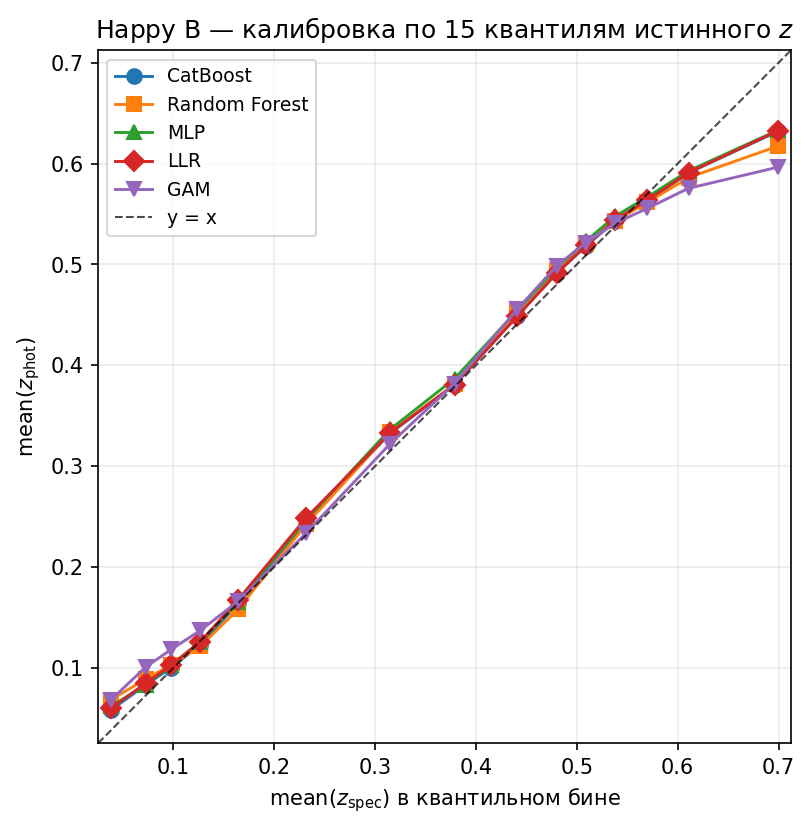
\includegraphics[width=\linewidth]{figures/calibration/calibration_happy_B.png}
\caption{HappyB}\label{fig:calib-happyB}
\end{subfigure}\hfill
\begin{subfigure}{0.32\textwidth}\centering
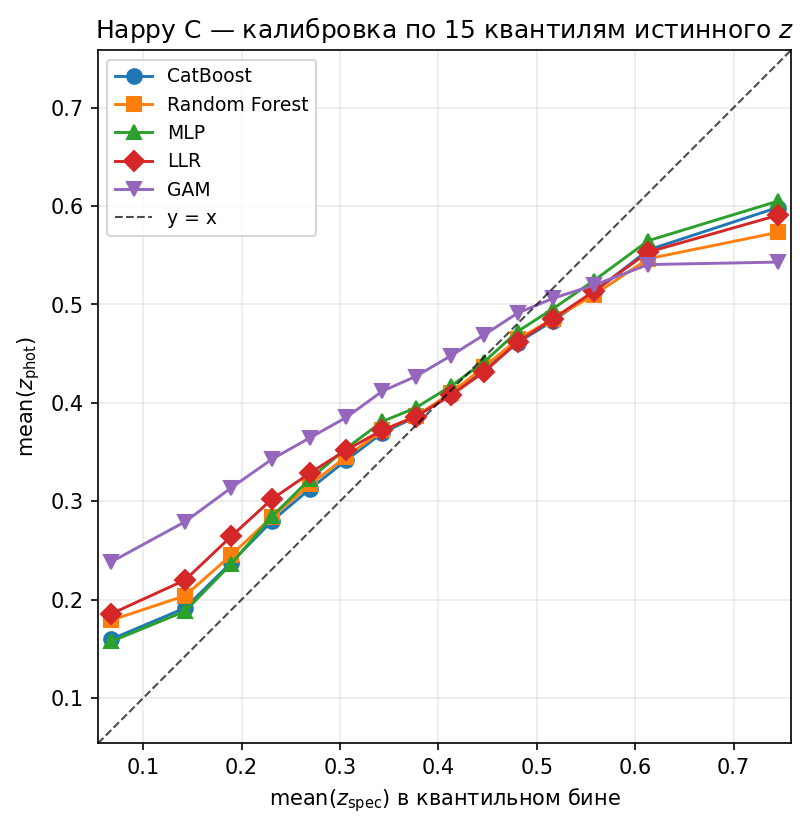
\includegraphics[width=\linewidth]{figures/calibration/calibration_happy_C.png}
\caption{HappyC}\label{fig:calib-happyC}
\end{subfigure}\hfill
\begin{subfigure}{0.32\textwidth}\centering
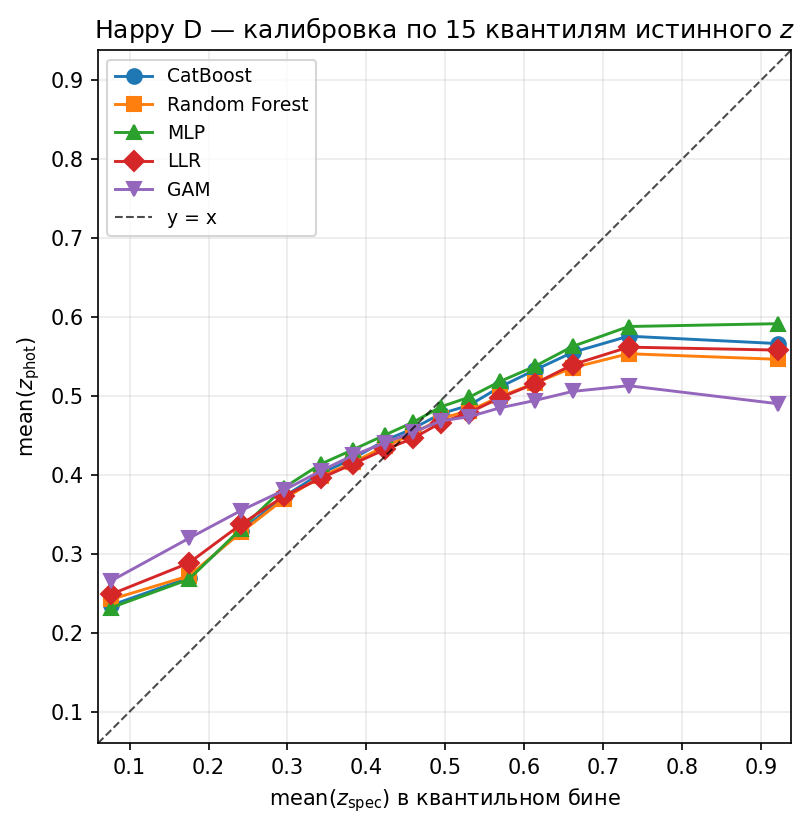
\includegraphics[width=\linewidth]{figures/calibration/calibration_happy_D.png}
\caption{HappyD}\label{fig:calib-happyD}
\end{subfigure}
\caption{Калибровочные кривые на подвыборках Happy.}
\label{fig:calib-happy}
\end{figure}

Калибровочные кривые выявляют третью системную проблему — смещение предсказаний к среднему (attenuation bias). На простых сплитах TeddyB, TeddyC и HappyB ломаные всех моделей близки к диагонали: модели хорошо откалиброваны в знакомом распределении. На TeddyD и HappyD наблюдается характерное отклонение: кривые уплощаются, завышая красное смещение у объектов с малыми истинными $z$ и занижая у объектов с большими. Это проявление эффекта, описанного в~\cite{ting2025}: модели систематически тяготеют к центру обучающего распределения и не обеспечивают надёжных предсказаний на краях. Эффект одинаково затрагивает все рассмотренные табличные методы и, по всей видимости, требует отдельной коррекции — калибровки предсказаний или целенаправленного взвешивания при обучении.

\clearpage
\section*{Заключение}
\addcontentsline{toc}{section}{Заключение}

В работе рассмотрена задача прогнозирования фотометрического красного смещения. Описаны факторы сложности задачи, наборы данных Teddy, Happy и SRGz, а также методы классического и глубокого обучения. Для воспроизводимого проведения экспериментов создан модульный стенд, объединяющий подготовку данных, обучение, применение моделей, расчёт метрик и генерацию отчётов.

Эксперименты выявили три системных ограничения рассматриваемых методов.

\textbf{Сдвиг распределения (Teddy).} На подвыборках TeddyB и TeddyC все табличные модели работают близко ($\sigma_{NMAD} \approx 0{,}017$). На TeddyD, где тестовое распределение существенно отличается от обучающего, CatBoost и Random Forest деградируют наиболее резко ($\sigma_{NMAD} \approx 0{,}076$–$0{,}079$), тогда как GAM оказывается наиболее устойчивым среди табличных методов ($\sigma_{NMAD} = 0{,}033$). Среди моделей на изображениях ConvNeXt-Tiny достигает сопоставимого уровня ($\sigma_{NMAD} = 0{,}035$), что подтверждает перспективность использования морфологической информации для работы в условиях сдвига распределения.

\textbf{Фотометрический шум и смещение по яркости (Happy).} При переходе от HappyB к HappyD $\sigma_{\mathrm{NMAD}}$ вырастает с $\approx 0{,}021$ до $\approx 0{,}081$ у CatBoost, MLP, LLR и RF; у GAM деградация ещё сильнее — с $0{,}033$ до $0{,}106$. GAM на всех сплитах Happy уступает остальным методам и демонстрирует наибольшую долю выбросов ($f_{\mathrm{outlier}} = 18{,}86\%$ на HappyD). Это свидетельствует о том, что данный тип деградации не связан с конкретной архитектурой и требует решений на уровне представления данных или аугментации.

\textbf{Смещение предсказаний к среднему (attenuation bias).} Калибровочные кривые на TeddyD и HappyD показывают характерное уплощение: модели завышают красное смещение у объектов с малыми истинными $z$ и занижают у объектов с большими. Этот эффект согласуется с наблюдением~\cite{ting2025} о том, что модели машинного обучения систематически тяготеют к центру обучающего распределения. Проблема одинаково затрагивает все рассмотренные табличные методы и требует отдельной калибровки предсказаний.

На прикладном каталоге SRGz все табличные модели показывают высокую долю выбросов (лучший результат у MLP: $f_{\mathrm{outlier}} = 14{,}17\%$), что отражает одновременное действие всех трёх перечисленных факторов.

Отдельно в работе идентифицирована четвёртая проблема — \emph{путаница близких по красному смещению скоплений галактик} (см. раздел~\ref{sec:photoz-challenges} и рисунок~\ref{fig:cluster-zou}). Типичное разрешение photo-z ($\sigma_z \sim 0{,}02$–$0{,}05$) превышает характерное расстояние между ближайшими скоплениями ($\Delta z \sim 0{,}01$), вследствие чего фотометрические каталоги не позволяют надёжно разделить членов соседних скоплений. Эта проблема иллюстрирована на реальных данных DESI, однако экспериментальная проверка методов её решения в рамках настоящей работы не проводилась и является самостоятельным направлением дальнейшего исследования.

Дальнейшая работа предполагает: отработку методов борьбы со сдвигом распределения и attenuation bias на Teddy и Happy; воспроизведение эксперимента с CapsNet в полной постановке; перенос наиболее удачных решений на SRGz с использованием изображений; а также разработку и тестирование подходов к разделению членов соседних скоплений на основе фотометрических красных смещений.

\bigskip
\noindent\textbf{Результаты, выносимые на защиту:}
\begin{enumerate}
    \item Разработан модульный экспериментальный стенд для сравнительного анализа классических и нейросетевых подходов к задаче фотометрического красного смещения. Стенд обеспечивает воспроизводимость, прозрачность и расширяемость экспериментов за счёт конфигурационного подхода, единого вычислительного пайплайна и унифицированного формата хранения артефактов и отчётов.
    \item Проведено сравнение пяти классических табличных моделей (CatBoost, Random Forest, MLP, LLR, GAM) и трёх архитектур глубокого обучения на изображениях (EfficientNet-B0, ConvNeXt-Tiny, ViT-Tiny) на наборах Teddy, Happy и SRGz. Показано, что при сдвиге распределения (TeddyD) ансамблевые методы CatBoost и Random Forest деградируют наиболее резко ($\sigma_{NMAD} \approx 0{,}076$–$0{,}079$), тогда как GAM является наиболее устойчивым табличным методом ($\sigma_{NMAD} = 0{,}033$). ConvNeXt-Tiny, обученный на изображениях, достигает сопоставимого уровня на TeddyD ($\sigma_{\mathrm{NMAD}} = 0{,}035$), уступая лучшему табличному методу (GAM, $0{,}033$) не более чем на $0{,}002$.
    \item Экспериментально подтверждены три системных ограничения рассматриваемых методов на задаче фотометрического красного смещения: деградация при сдвиге обучающего распределения, нарастающая от сплита к сплиту деградация под действием фотометрического шума и смещения по яркости, а также систематическое смещение предсказаний к среднему (attenuation bias), проявляющееся в уплощении калибровочных кривых при переходе к сложным сплитам.
    \item Идентифицирована и проиллюстрирована на реальных данных DESI четвёртая прикладная проблема — невозможность надёжного разделения членов близких по красному смещению скоплений галактик средствами photo-z. Типичное разрешение фотометрических методов ($\sigma_z \sim 0{,}02$–$0{,}05$) превышает характерное расстояние между соседними скоплениями ($\Delta z \sim 0{,}01$), что проявляется в сохранении ложных пиков на гистограмме $N(z)$ даже после геометрической вырезки соседних скоплений.
\end{enumerate}

\newpage
\begin{thebibliography}{99}
\addcontentsline{toc}{section}{Литература}

\bibitem{newman2022}
Newman J. A., Gruen D. Photometric Redshifts for Next-Generation Surveys // Annual Review of Astronomy and Astrophysics. 2022. Vol. 60. P. 363–414. DOI: 10.1146/annurev-astro-032122-014611.

\bibitem{meshcheryakov2022}
Мещеряков А. В., Машечкин И. В., Герасимов С. В. и др. SRGz: методы машинного обучения и свойства каталога оптических компаньонов точечных рентгеновских источников СРГ/eROSITA в области покрытия DESI Legacy Imaging Surveys // Письма в Астрономический журнал. 2023. Т. 49. № 7. С. 441–494. DOI: 10.31857/S0320010823070021.

\bibitem{beck2017}
Beck R., Lin C.-A., Ishida E. E. O. et al. On the realistic validation of photometric redshifts, or why Teddy will never be Happy // Monthly Notices of the Royal Astronomical Society. 2017. Vol. 468. No. 4. P. 4323–4337. DOI: 10.1093/mnras/stx687.

\bibitem{ting2025}
Ting Y.-S. Why Machine Learning Models Systematically Underestimate Extreme Values // The Open Journal of Astrophysics. 2025. Vol. 8.

\bibitem{dorogush2018catboost}
Dorogush A. V., Ershov V., Gulin A. CatBoost: gradient boosting with categorical features support. 2018. arXiv:1810.11363.

\bibitem{breiman2001randomforest}
Breiman L. Random Forests // Machine Learning. 2001. Vol. 45. No. 1. P. 5–32. DOI: 10.1023/A:1010933404324.

\bibitem{tan2019efficientnet}
Tan M., Le Q. V. EfficientNet: Rethinking Model Scaling for Convolutional Neural Networks // Proceedings of the 36th International Conference on Machine Learning. 2019. P. 6105–6114.

\bibitem{liu2022convnext}
Liu Z., Mao H., Wu C.-Y., Feichtenhofer C., Darrell T., Xie S. A ConvNet for the 2020s // Proceedings of the IEEE/CVF Conference on Computer Vision and Pattern Recognition. 2022. P. 11976–11986.

\bibitem{dosovitskiy2020vit}
Dosovitskiy A., Beyer L., Kolesnikov A. et al. An Image is Worth 16x16 Words: Transformers for Image Recognition at Scale // International Conference on Learning Representations. 2021. arXiv:2010.11929.

\bibitem{dey2022}
Dey B., Andrews B. H., Newman J. A., Mao Y.-Y., Rau M. M., Zhou R. Photometric redshifts from SDSS images with an interpretable deep capsule network // Monthly Notices of the Royal Astronomical Society. 2022. Vol. 515. No. 4. P. 5285–5305. DOI: 10.1093/mnras/stac2105.

\bibitem{sabour2017capsnet}
Sabour S., Frosst N., Hinton G. E. Dynamic Routing Between Capsules // Advances in Neural Information Processing Systems. 2017. Vol. 30. P. 3856–3866.

\bibitem{rajasegaran2019deepcaps}
Rajasegaran J., Jayasundara V., Jayasekara S., Jayasekara H., Seneviratne S., Rodrigo R. DeepCaps: Going Deeper with Capsule Networks // Proceedings of the IEEE/CVF Conference on Computer Vision and Pattern Recognition. 2019. P. 10725–10733.

\end{thebibliography}

\newpage
\appendix

\setcounter{figure}{0}
\renewcommand{\thefigure}{А.\arabic{figure}}
\section*{\centering Приложение А}
\phantomsection
\addcontentsline{toc}{section}{Приложение А. Распределения подвыборок Teddy}

\begin{center}
    \large Распределения подвыборок Teddy
\end{center}

\begin{figure}[H]
    \centering
    \includegraphics[width=\textwidth]{figures/teddy_distribution.png}
    \caption{Распределения для набора Teddy. Иллюстрация показывает сдвиг распределения между обучающей подвыборкой A и тестовыми подвыборками B, C и D.}
    \label{fig:teddy-distribution}
\end{figure}

\newpage
\setcounter{figure}{0}
\renewcommand{\thefigure}{Б.\arabic{figure}}
\section*{\centering Приложение Б}
\phantomsection
\addcontentsline{toc}{section}{Приложение Б. Распределения подвыборок Happy}

\begin{center}
    \large Распределения подвыборок Happy
\end{center}

\begin{figure}[H]
    \centering
    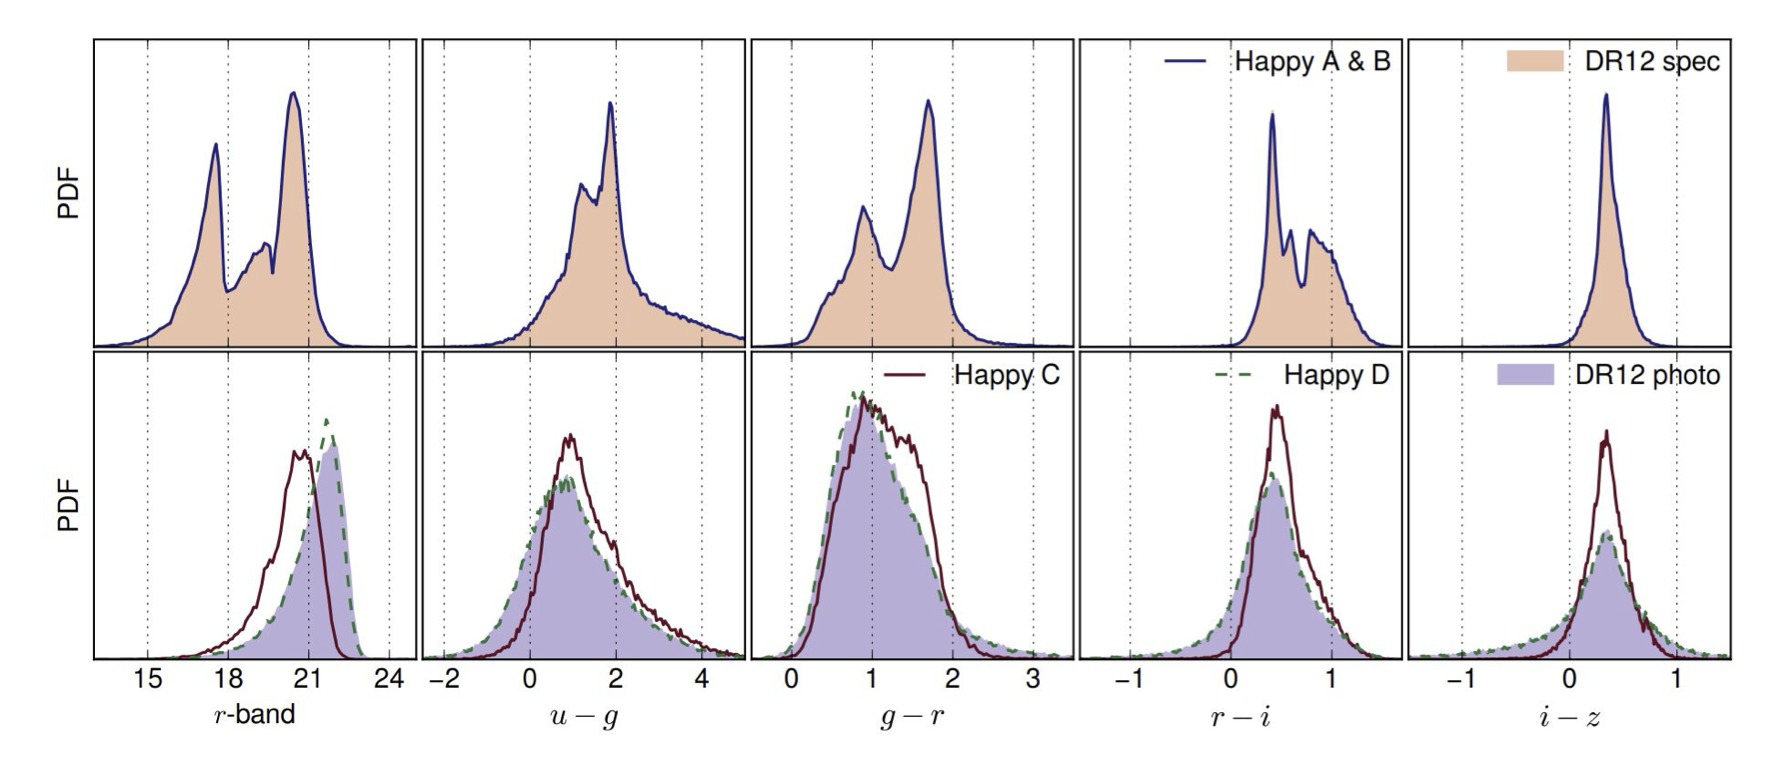
\includegraphics[width=\textwidth]{figures/happy_distribution.png}
    \caption{Распределения для набора Happy. Иллюстрация отражает перенос модели с более ярких объектов на более слабые и более шумные подвыборки.}
    \label{fig:happy-distribution}
\end{figure}

\end{document}
